\documentclass[letter,12pt]{article}
\usepackage[paperheight=27.94cm,paperwidth=21.59cm,bindingoffset=0in,left=3cm,right=2.0cm, top=3.5cm,bottom=2.5cm, headheight=200pt, headsep=1.0\baselineskip]{geometry}
\usepackage{graphicx,lastpage}
\usepackage{upgreek}
\usepackage{censor}
\usepackage[spanish,es-tabla]{babel}
\usepackage{pdfpages}
\usepackage{tabularx}
\usepackage{graphicx}
\usepackage{adjustbox}
\usepackage{xcolor}
\usepackage{colortbl}
\usepackage{rotating}
\usepackage{multirow}
\usepackage[utf8]{inputenc}
\usepackage{float}
\usepackage{hyperref}
\usepackage{listings}
\lstdefinelanguage{YAML}{
  keywords={true,false,null,y,n},
  sensitive=false,
  comment=[l]{\#},
  morecomment=[s]{/*}{*/},
  morestring=[b]',
  morestring=[b]"
}
\lstdefinelanguage{bash}{
  morekeywords={curl,echo,grep,awk,sed,cat,ls,cd,mkdir,rm,docker},
  sensitive=true,
  morecomment=[l]{\#},
  morestring=[b]",
}
\lstset{
  basicstyle=\ttfamily\small,
  numbers=left,
  numberstyle=\tiny\color{gray},
  frame=single,
  breaklines=true,
  postbreak=\mbox{\textcolor{red}{$\hookrightarrow$}\space},
  captionpos=b,
  keywordstyle=\color{blue}\bfseries,
  commentstyle=\color{gray}\itshape,
  stringstyle=\color{orange},
}

\renewcommand{\tablename}{Tabla}
\usepackage{fancyhdr}
\pagestyle{fancy}

\fancyhead[L]{}
%
\begin{document}
%
   \title{\Huge{Informe Laboratorio 2}}

   \author{\textbf{Sección 1} \\  \\Alumno Diego Banda Gálvez \\ e-mail: diego.banda@mail.udp.cl}
          
   \date{Septiembre de 2025}

   \maketitle
   
   \tableofcontents
 
  \newpage
  

\section{Descripción de actividades}
Utilizando la aplicación web vulnerable DVWA

(Damn Vulnerable Web App - \href{https://github.com/digininja/DVWA}{https://github.com/digininja/DVWA} (Enlaces a un sitio externo.)) realice las siguientes actividades:


\begin{itemize}
    \item Despliegue la aplicación en su equipo utilizando docker. Detalle el procedimiento y explique los parámetros que utilizó.
    \item Utilice Burpsuite (https://portswigger.net/burp/communitydownload (Enlaces a un sitio externo.)) para realizar un ataque de fuerza bruta contra formulario ubicado en vulnerabilities/brute. Explique el proceso y obtenga al menos 2 pares de usuario/contraseña válidos. Muestre las diferencias observadas en burpsuite.
    \item Utilice la herramienta cURL, a partir del código obtenido de inspect elements de su navegador, para realizar un acceso válido y uno inválido al formulario ubicado en vulnerabilities/brute. Indique 4 diferencias entre la página que retorna el acceso válido y la página que retorna un acceso inválido.
    \item Utilice la herramienta Hydra para realizar un ataque de fuerza bruta contra formulario ubicado en vulnerabilities/brute. Explique el proceso y obtenga al menos 2 pares de usuario/contraseña válidos.
    \item Compare los paquetes generados por hydra, burpsuite y cURL. ¿Qué diferencias encontró? ¿Hay forma de detectar a qué herramienta corresponde cada paquete?

    \item Desarrolle un script en Python para realizar un ataque de fuerza bruta:

    \begin{itemize}
        \item Utilice la librería requests para interactuar con el formulario ubicado en vulnerabilities/brute y desarrollar su propio script de fuerza bruta en Python.
        El script debe realizar intentos de inicio de sesión probando una lista de combinaciones de usuario/contraseña.

        \item  Identifique y explique la cabecera HTTP que empleará para realizar el ataque de fuerza bruta.

        \item  Muestre el código y los resultados obtenidos (al menos 2 combinaciones válidas de usuario/contraseña).

        \item Compare el rendimiento de este script en Python con las herramientas Hydra, Burpsuite, y cURL en términos de velocidad y detección.
    \end{itemize}

    \item  Investigue y describa 4 métodos comunes para prevenir o mitigar ataques de fuerza bruta en aplicaciones web:

    \begin{itemize}
        \item Para cada método, explique su funcionamiento, destacando en qué escenarios es más eficaz.

    \end{itemize}


    
\end{itemize}

\section{Desarrollo de actividades según criterio de rúbrica}

\subsection{Levantamiento de docker para correr DVWA (dvwa)}

A través del mismo github entregado de DVWA, en su README, se encuentran distintas maneras de levantar el servicio, principalmente dos, la primera descargando el servicio para luego a través de comandos propios levantarlo, sin embargo en este desarrollo se decidió optar por su levantamiento a través de docker.
Esta opción entrega una forma más sencilla y rápida de levantar el servicio, primero descargando la imagen oficial, para luego a través de un \textit{docker-compose.yml} tener la configuración inicial y a través de este realizar el levantamiento.

Inicialmente se descarga la imagen con:
\begin{lstlisting}[language=bash, caption={Descarga de imagen}]
docker pull ghcr.io/digininja/dvwa:c6e3d05
\end{lstlisting}
Una vez con la imagen, se crea el \textit{docker-compose.yml}:
\begin{lstlisting}[language=YAML, caption={\textit{docker-compose.yml} para DVWA}]
services:
  web:
    image: vulnerables/web-dvwa:latest
    container_name: dvwa_web
    ports:
      - "4280:80"
    restart: always
\end{lstlisting}
Los parámetros vistos corresponden a lo siguiente:
\begin{itemize}
    \item \textbf{'web':} Nombre asignado en archivo, en caso de requerir levantar otros a través del mismo \textit{docker-compose-yml}.
    \item \textbf{image:} La imagen de DVWA descargada, indicando que es la a utilizar.
    \item \textbf{container\_name:} El nombre asignado al contenedor una vez levantado el servicio.
    \item \textbf{ports:} El mapeo de puertos a utilizar, en este caso el puerto local del computador 4280 se está mapeando al que utiliza la aplicación (80).
    \item \textbf{restart:} Este parámetro está en caso de posibles problemas con el contenedor, ante una posible falla y caída del contenedor, este se intentará volver a levantar automáticamente.
\end{itemize}

Una vez tengamos lo anterior listo, tan solo basta con ejecutar el siguiente comando a través de la terminar en la misma carpeta.
\begin{lstlisting}[language=bash, caption={Levantamiento de contenedor}]
docker compose up -d
\end{lstlisting}
\begin{figure}[H]
    \centering
    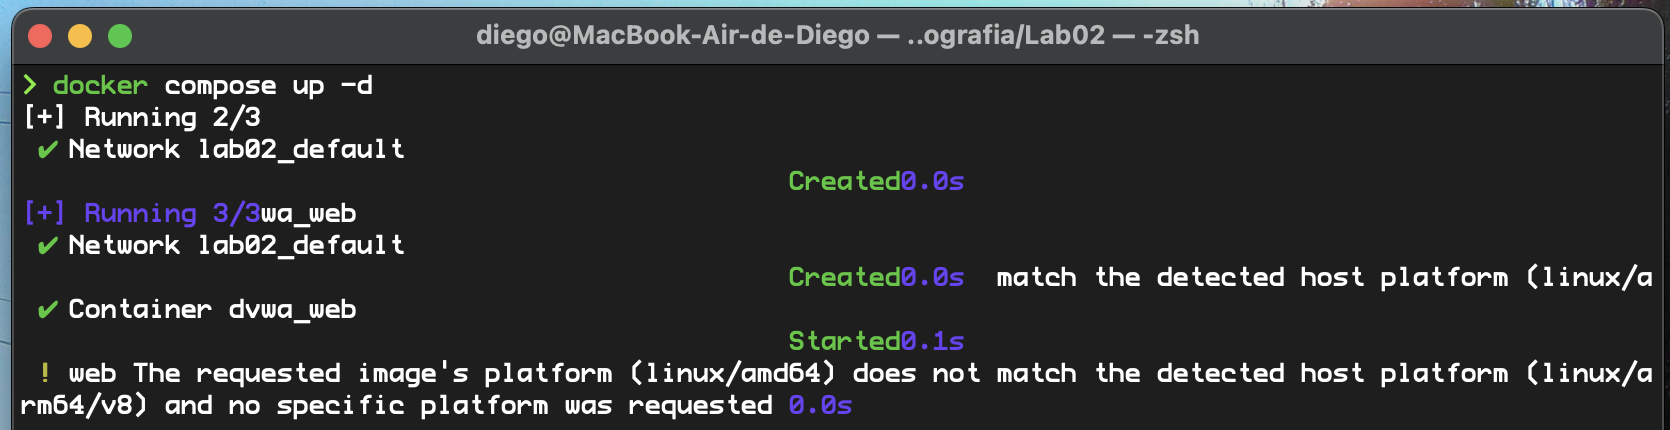
\includegraphics[width=1\linewidth]{Imagenes/docker_compose_up.png}
    \caption{funcionamiento y output de \textit{docker compose up -d}}
    \label{fig:placeholder}
\end{figure}
La advertencia que aparece es porque todo este procedimiento se está realizando en una computadora MacBoock Air M1, y la aplicación fue desarrollada principalmente para sistemas Linux.

\subsection{Redirección de puertos en docker (dvwa)}

La aplicación internamente trabaja a través del puerto 80 por ser una aplicación web (http), sin embargo gracias a docker y su docker compose, esto se puede modificar según posibles necesidades, problemas o comodidad.
Esto se realiza a través de nuestro \textit{docker-compose.yml}, en el parámetro "ports" se redirecciona el puerto 80 de la aplicación a uno de decisión propia, en el archivo presentado en el ítem anterior se mapea tal puerto 80 a nuestro puerto 4280, de esta manera, si se quiere realizar una conexión a la aplicación, esta se debe realizar a través del puerto mencionado.
Si se requiere cambiar de puerto a utilizar nuevamente, es tan sencillo cómo cambiar tal configuración en el archivo correspondiente, y reiniciar el contenedor en caso de estar funcionando.

\subsection{Obtención de consulta a replicar (burp)}

Con el sitio levantado en \textit{localhost:4280}, se puede acceder a este, obteniendo inicialmente una página de login, con la cual utilizamos las contraseñas \textit{default} (username: admin, Password: password), una vez dentro, se debe crear/reiniciar la base de datos, para luego pasar a volver al login y ahora sí entrar a la aplicación web con todas sus funcionalidades.

Dentro de esta página web se tiene entre sus apartados de vulnerabilities, Brute Force, el cual consta del típico formulario utilizado para realizar un inicio de sesión en páginas web.
\begin{figure}[H]
    \centering
    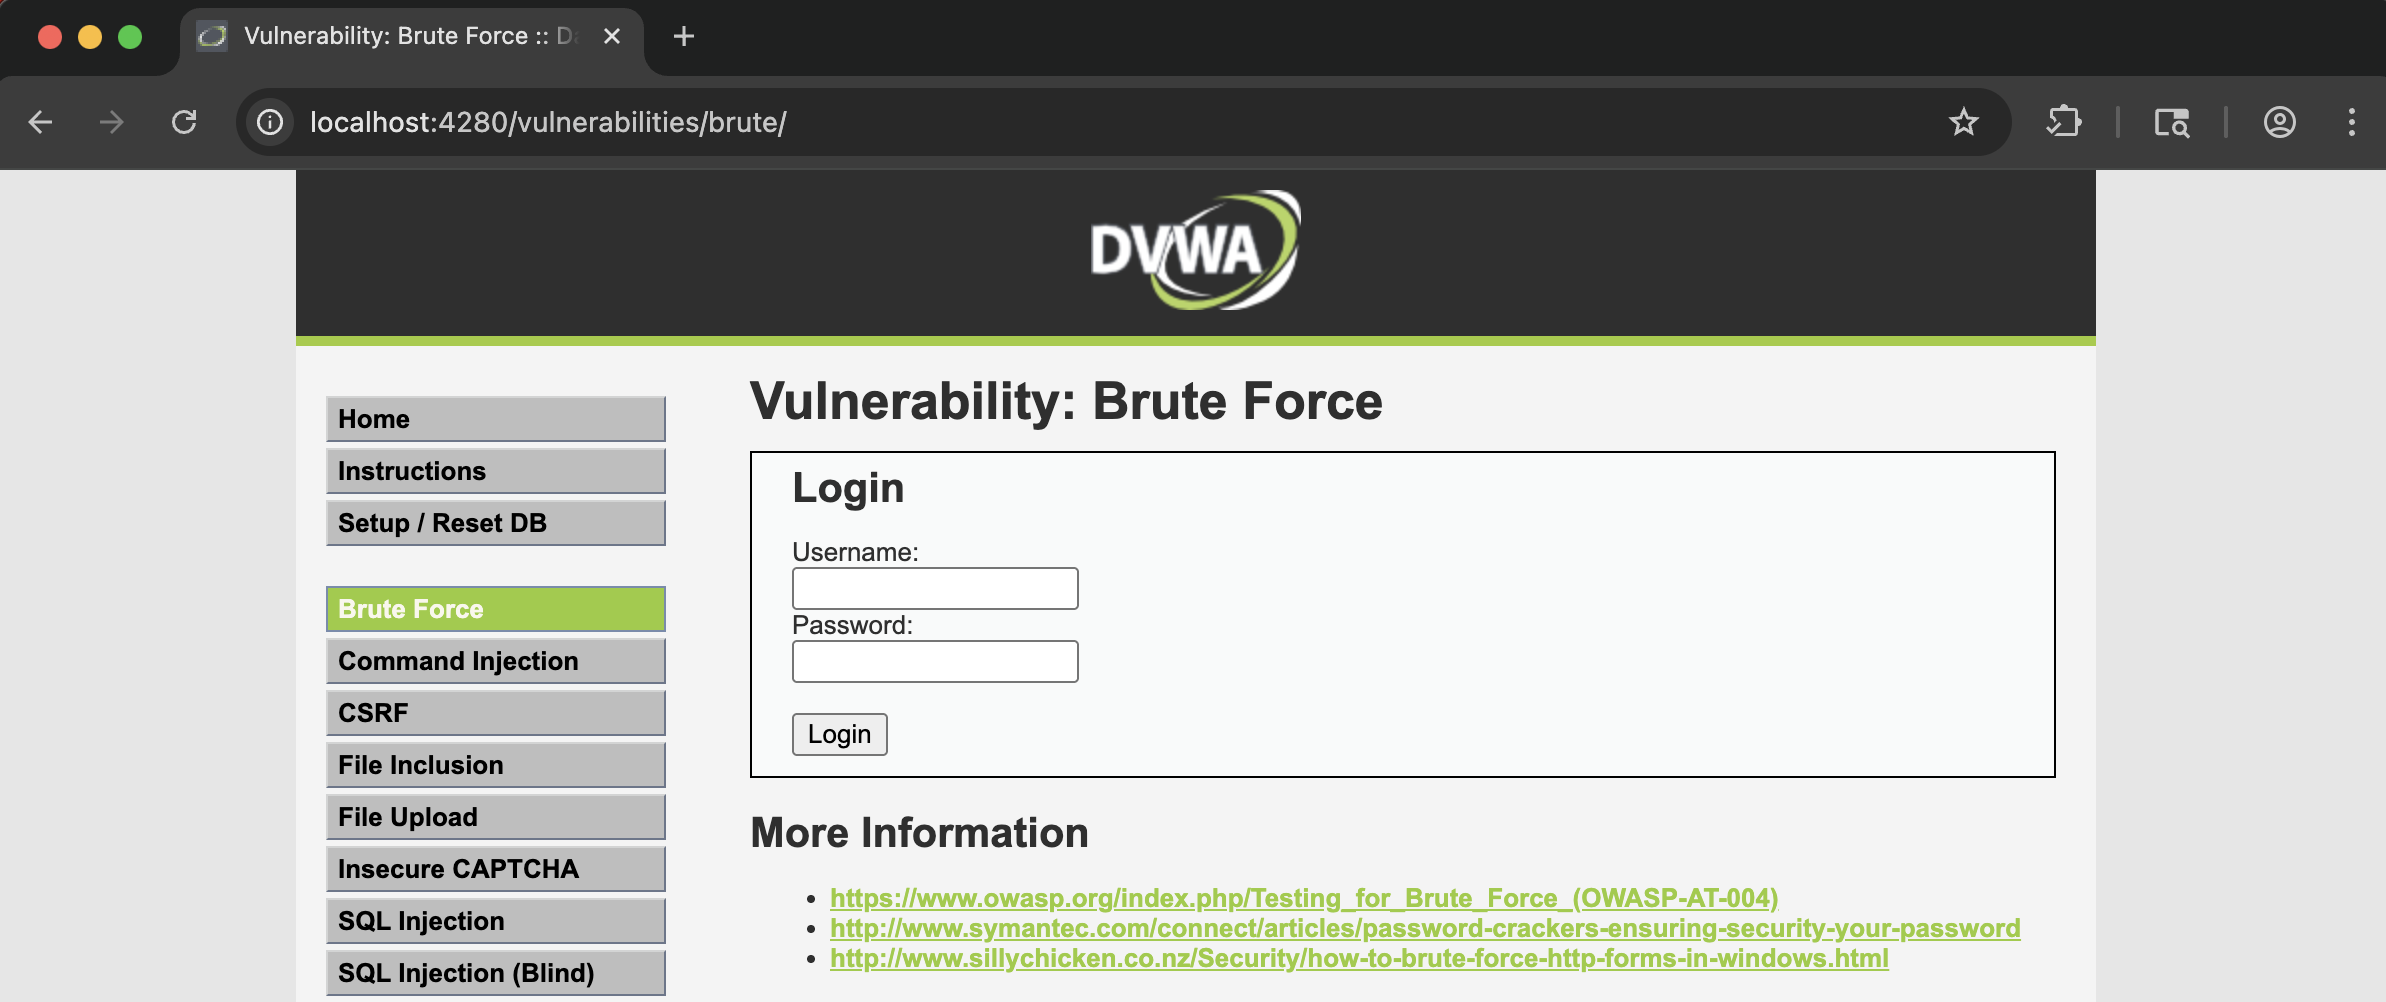
\includegraphics[width=0.75\linewidth]{Imagenes/brute_force_form.png}
    \caption{Formulario de inicio de sesión Brute Force}
    \label{fig:placeholder}
\end{figure}

A través de la pestaña 'target' de burp suite y su propio navegador incorporado (chromium) se hace una petición POST con tal formulario mencionado anteriormente y se captura lo enviado y lo recibido, de esta manera se realiza un análisis sobre de qué manera se está realizando la comunicación.
\begin{figure}[H]
    \centering
    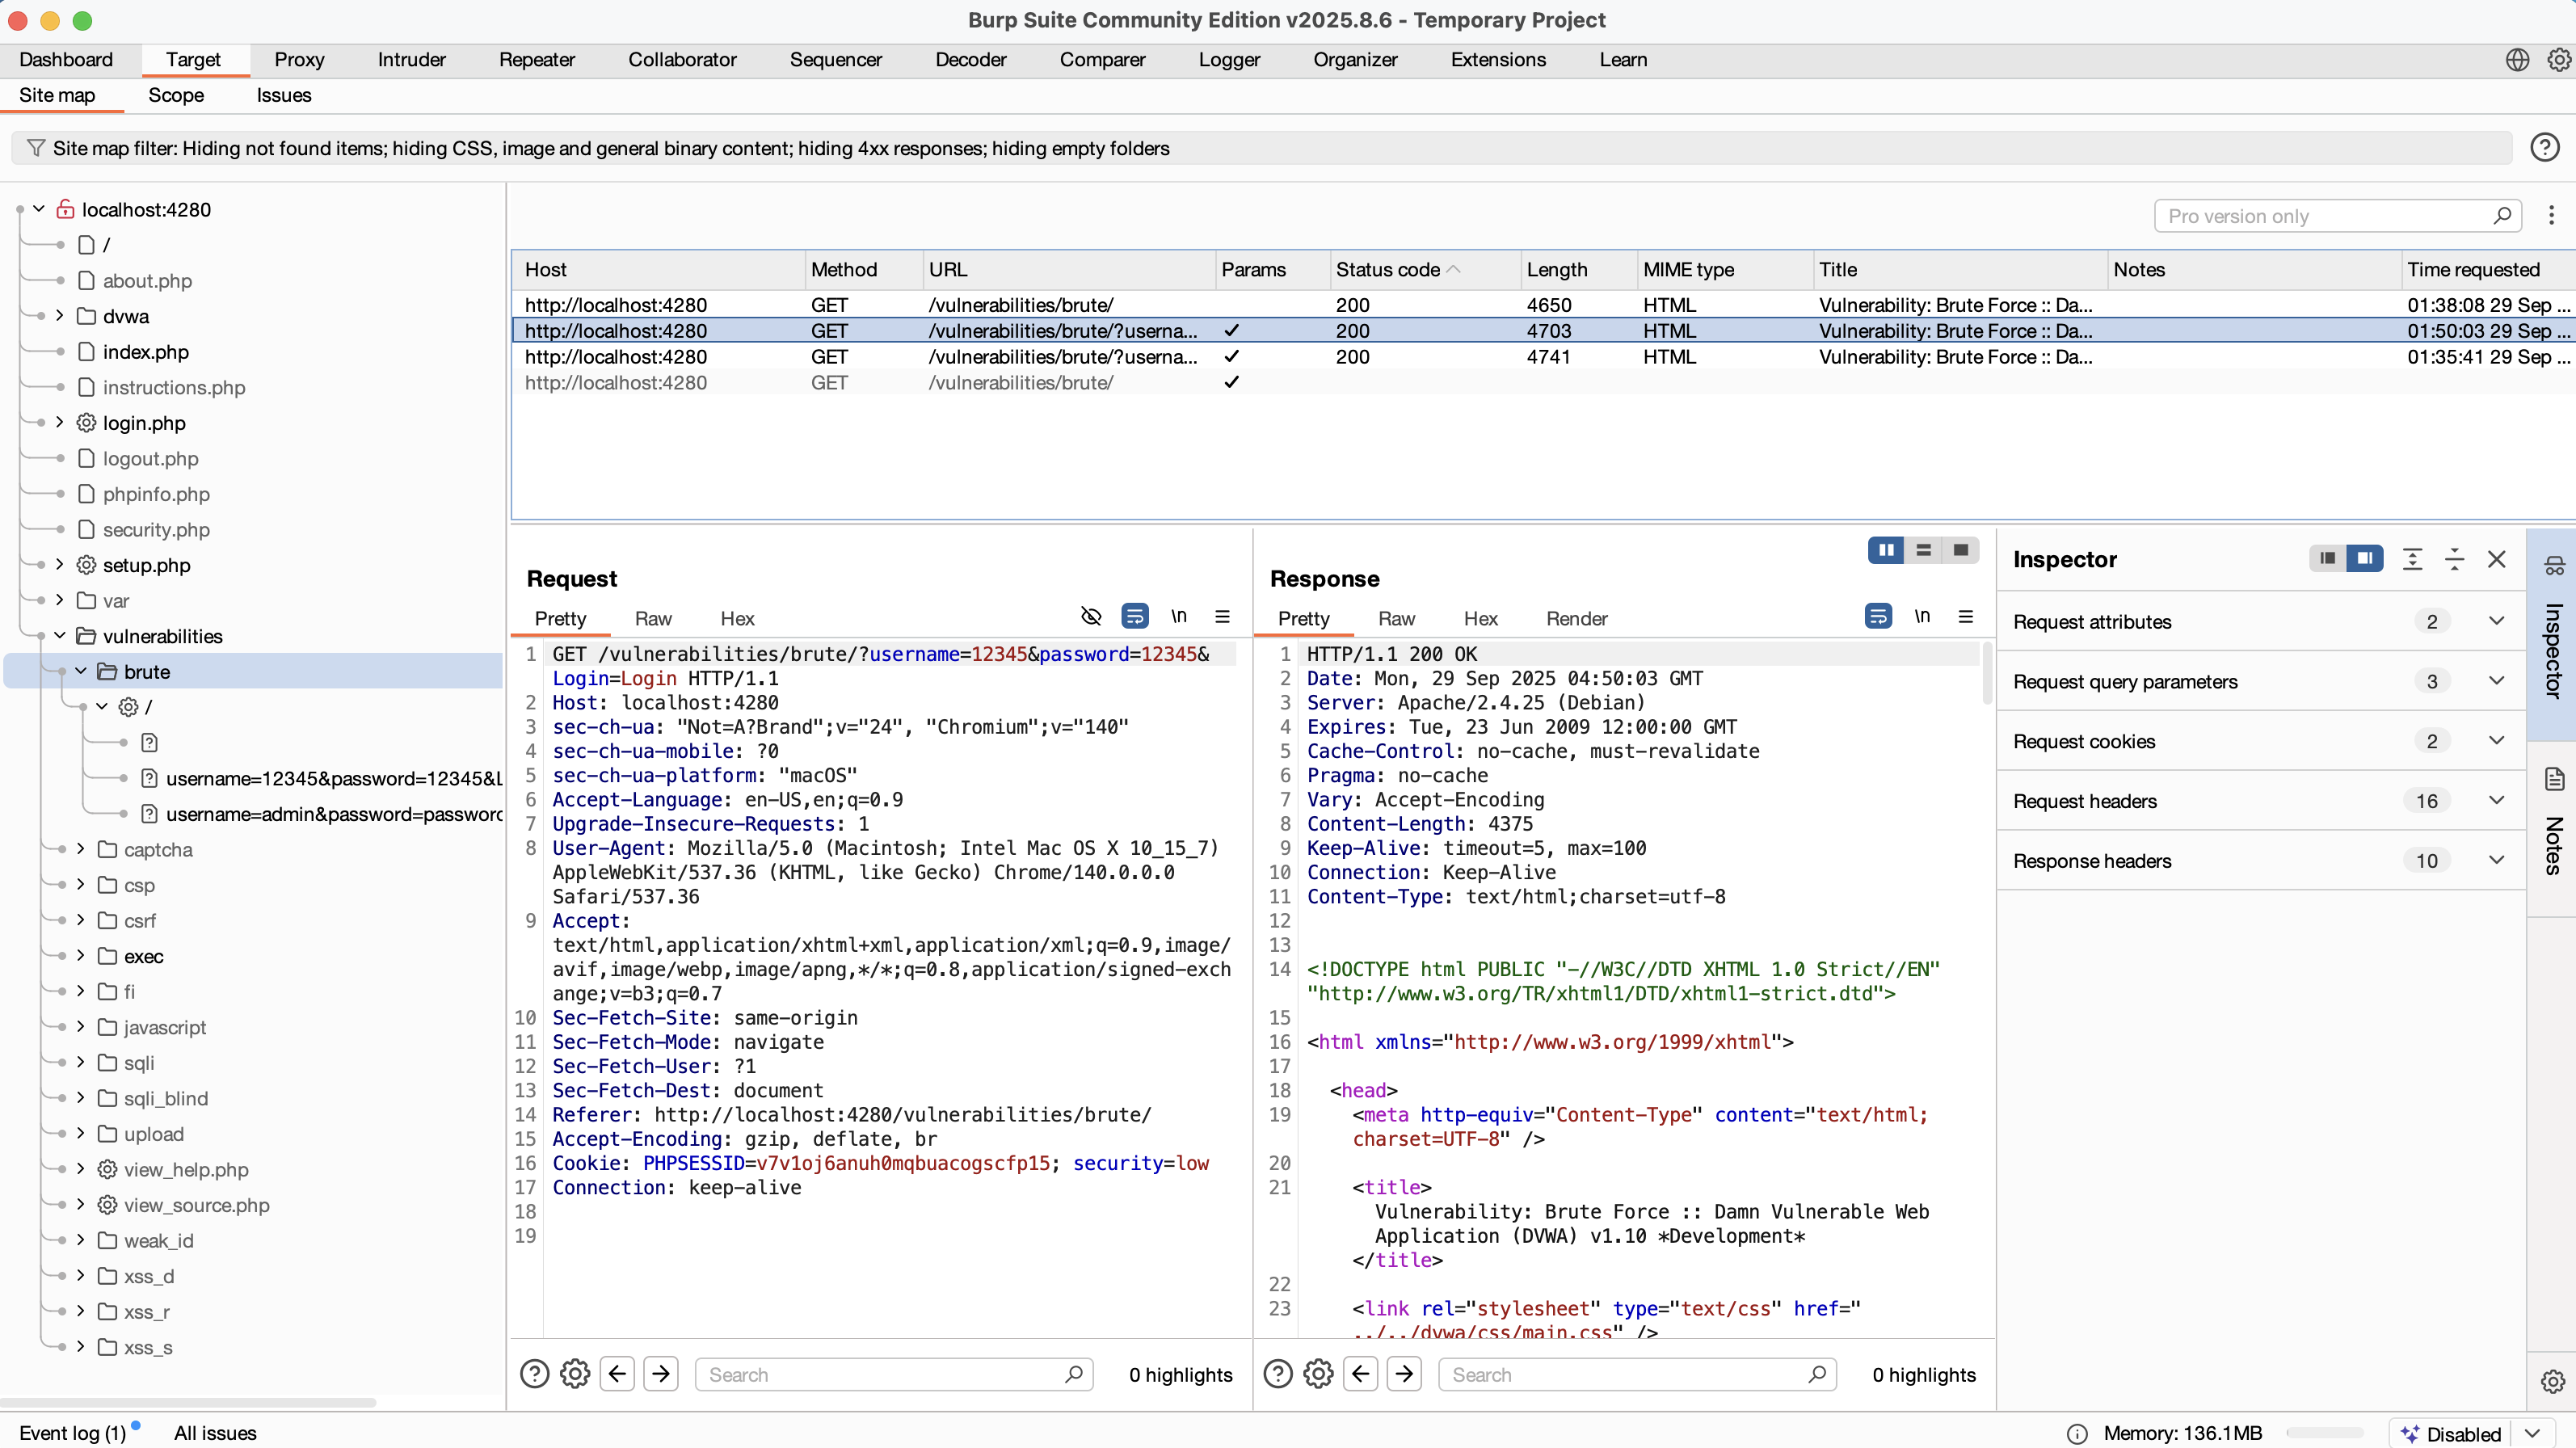
\includegraphics[width=1\linewidth]{Imagenes/brute_force_inicial_capture.png}
    \caption{Captura inicial de peticiones}
    \label{fig:placeholder}
\end{figure}

Como se puede observar en 'Request', se está haciendo envío de ambos parámetros en la primera línea de este GET, esta petición se usará como base para replicarla con distintos parámetros y lograr nuestro ataque de fuerza bruta.

\subsection{Identificación de campos a modificar (burp)}

Ya teniendo la consulta que se replicará, esta se envía a la pestaña 'Intruder' de burp, la cual sirve para realizar ataques de fuerza bruta o 'Cluster bomb attack', los cuales consisten en probar todas las combinaciones posibles de datos desde un diccionario para comprobar si alguna de estas combinaciones efectivamente accede al sitio web.

Desde la petición se deben identificar los parámetros que se envían, el formulario al solamente tener username y password, se debe de buscar ambos en la petición (y posibles réplicas).
Afortunadamente en esta petición se encuentran ambos parámetros en la primera línea, por lo tanto con la misma herramienta mencionada anteriormente se seleccionan (los valores después de 'username' y 'password') y marcan como payload.
\begin{figure}[H]
    \centering
    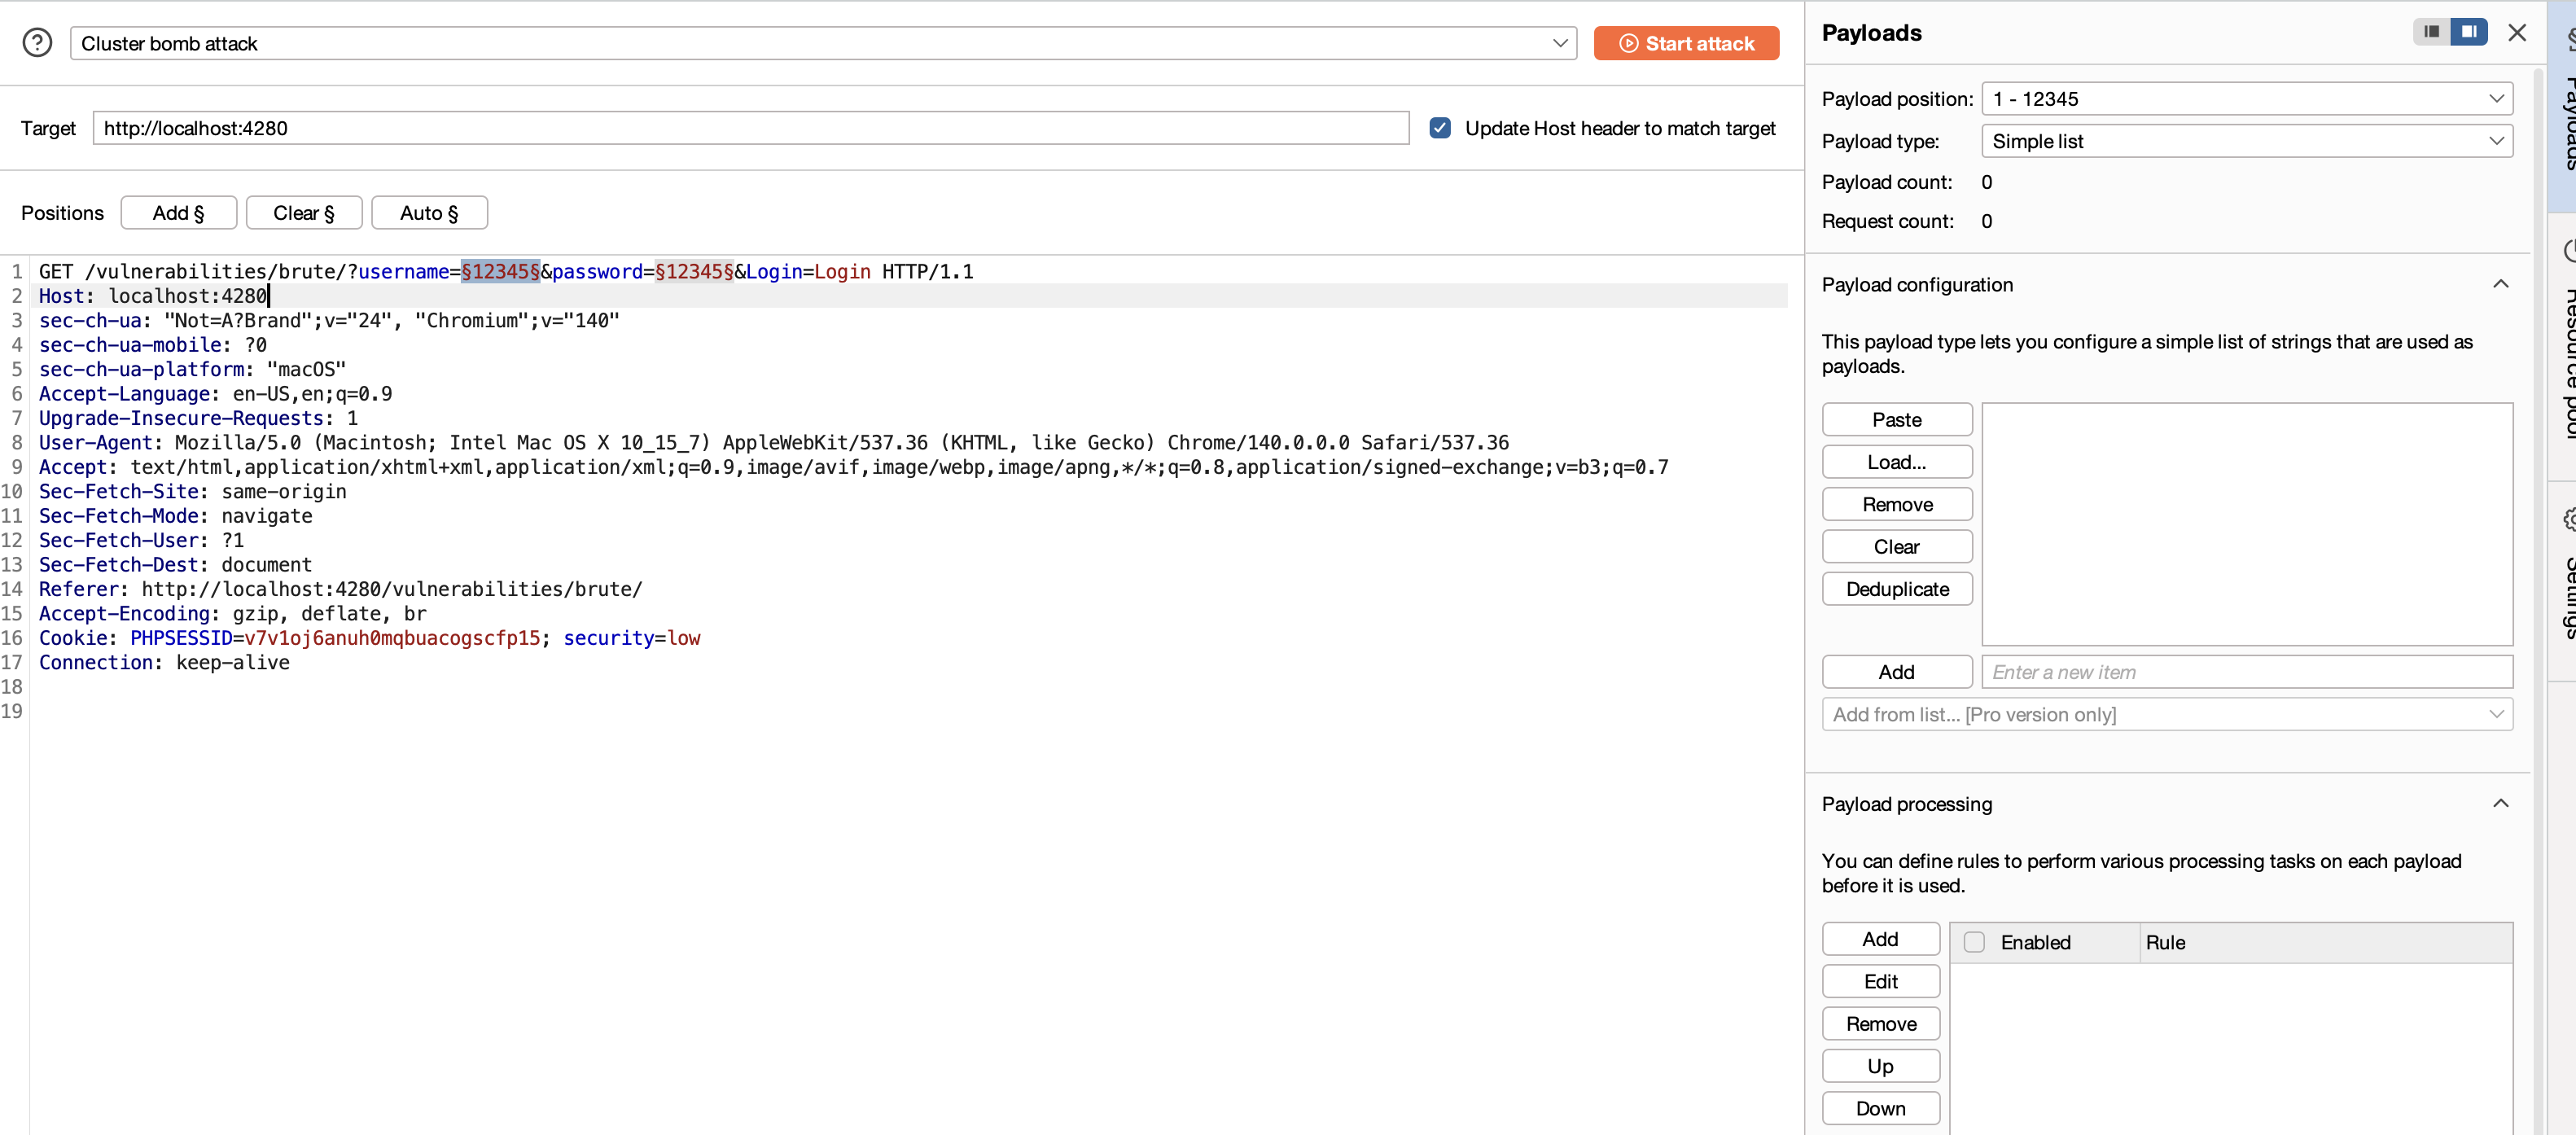
\includegraphics[width=1\linewidth]{Imagenes/brute_force_parameters.png}
    \caption{Identificación de parámetros}
    \label{fig:placeholder}
\end{figure}

\subsection{Obtención de diccionarios para el ataque (burp)}

Para realizar un ataque de fuerza bruta es necesario un diccionario, un diccionario es una lista de posibles usernames o password que se deberán probar en el inicio de sesión.
Teniendo estas dos listas por separado se intentan cada una de las combinaciones verificando que se logre un inicio de sesión.

Es importante contar con buenos diccionarios para llegar a buen puerto, ya que nuestro posible par usuario contraseña buscado debe estar dentro de estos diccionarios, por lo tanto mientras más representativos sean, mejor.
Con más representativos me refiero a datos más comúnmente utilizados y una gran cantidad de estos, mientras más combinaciones se prueben, mejor será nuetro ataque.

Burpsuite es una herramienta bastante limitada (sobre todo su versión gratuita), por lo tanto es un problema utilizar diccionarios demasiado grandes, porque gracias a su velocidad limitada tomará demasiado tiempo en encontrar la o las contraseñas, es por ello que para usuarios se utilizó una pequeña modificación de \textit{top-usernames-shortlist.txt} (\href{https://github.com/danielmiessler/SecLists/blob/master/Usernames/top-usernames-shortlist.txt}{link}) (se le agregaron los usernames: gordonb, 1337, user, pablo, smithy ya que se identificó que estaban presentes en la base de deatos) y para contraseñas se utilzó \textit{Pwdb\_top-1000.txt} (\href{https://github.com/danielmiessler/SecLists/blob/master/Passwords/Common-Credentials/Pwdb_top-1000.txt}{link})

\subsection{Obtención de al menos 2 pares (burp)}

Un ataque de fuerza bruta, como se mencionó anteriormente, consta de probar todas las combinaciones del par username password del diccionario, en la pestaña 'Intruder' abierta anteriormente se realizan las configuraciones necesarias:
\begin{itemize}
    \item \textbf{Payload 1:} Se le asignan los valores de \textit{top-usernames-shortlist.txt}
    \begin{figure}[H]
        \centering
        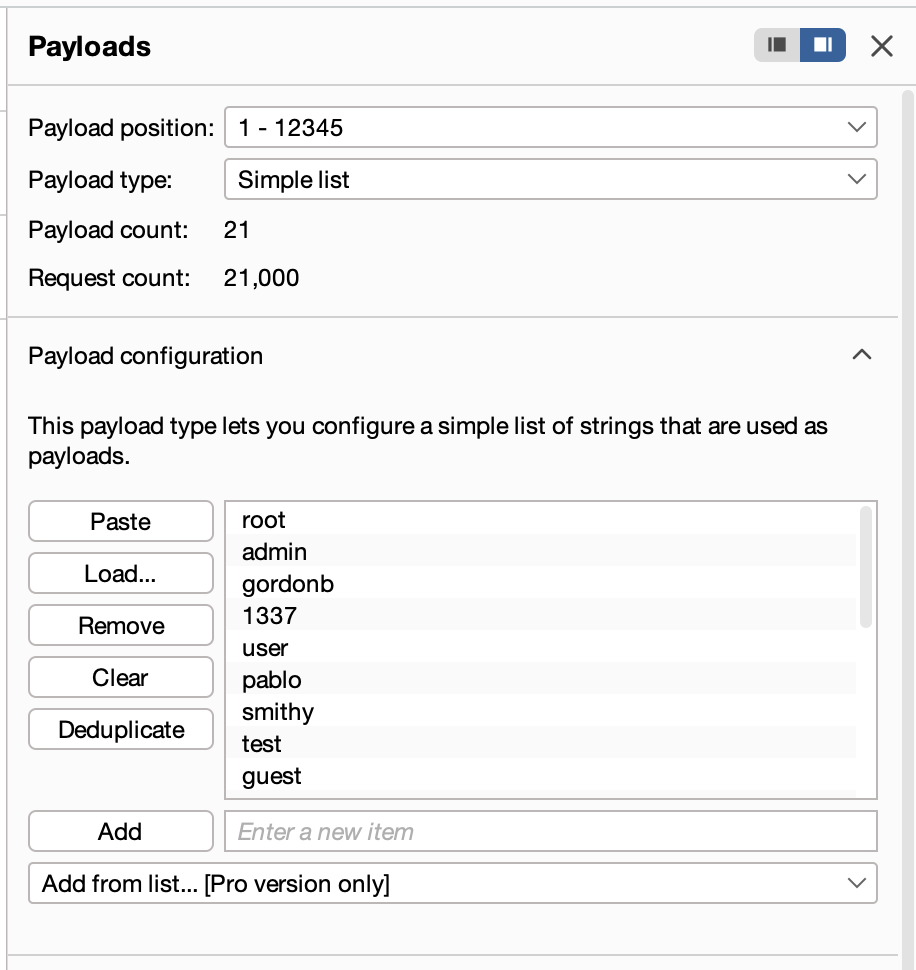
\includegraphics[width=0.5\linewidth]{Imagenes/brute_force_payload1.png}
        \caption{Payload 1}
        \label{fig:placeholder}
    \end{figure}
    \item \textbf{Payload 2:} Se le asignan los valores de \textit{Pwdb\_top-1000.txt}.
    \begin{figure}[H]
        \centering
        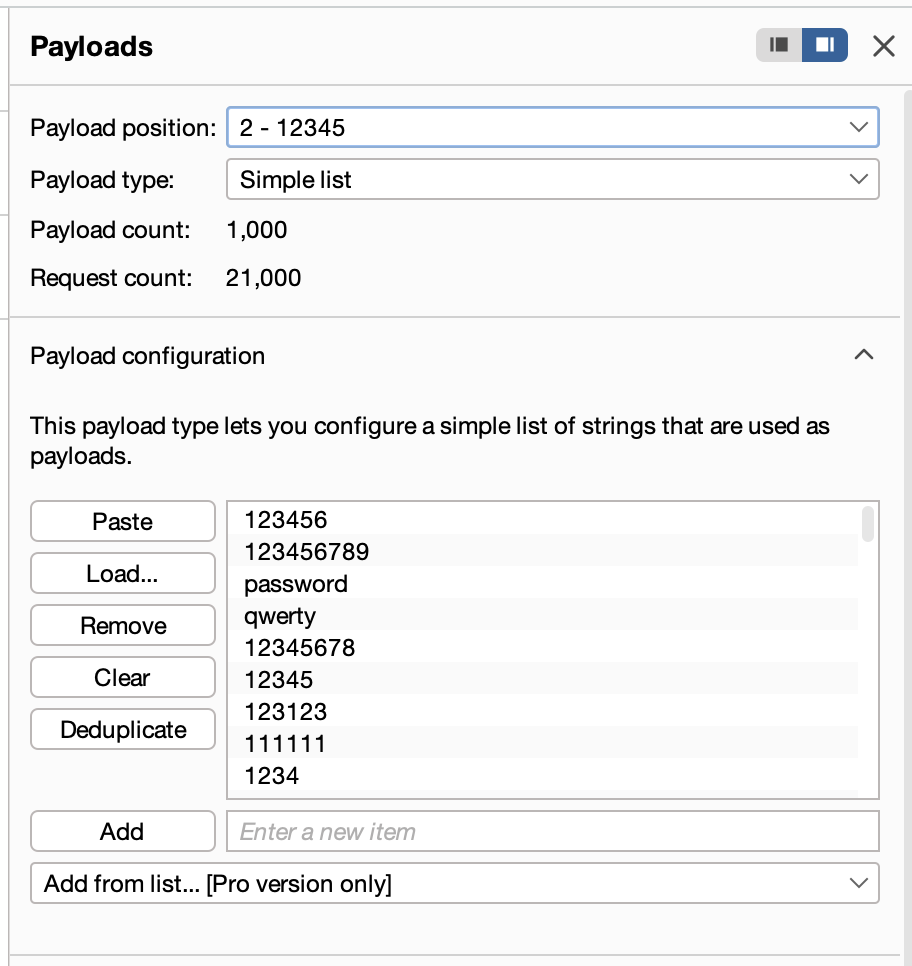
\includegraphics[width=0.5\linewidth]{Imagenes/brute_force_payload2.png}
        \caption{Payload 2}
        \label{fig:placeholder}
    \end{figure}
    \item \textbf{Settings:} Se activa y eliminan los valores predeterminados de \textit{Grep - Match}, para luego agregar la palabra \textit{incorrect}, de esta manera se identifican todos los intentos fallidos y se diferencian los correctos.
    \begin{figure}[H]
        \centering
        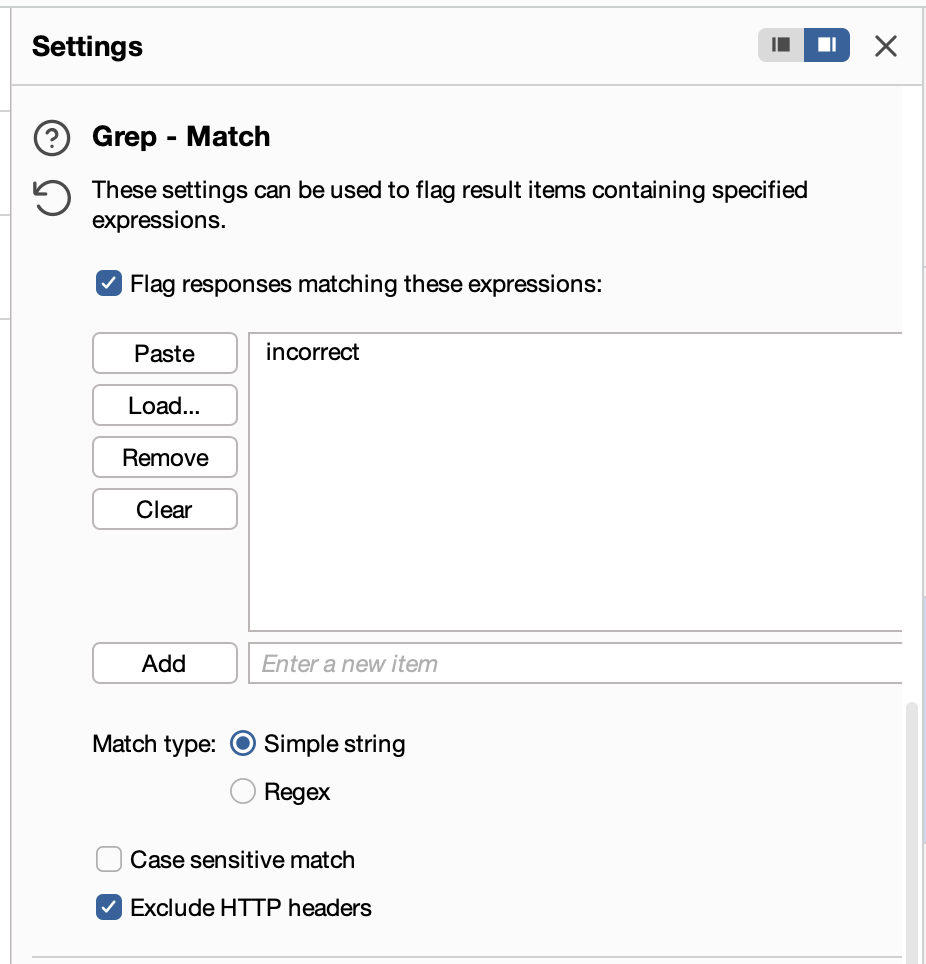
\includegraphics[width=0.5\linewidth]{Imagenes/brute_force_settings_match.png}
        \caption{Settings Grep - Match}
        \label{fig:placeholder}
    \end{figure}
\end{itemize}
Una vez estas configuraciones están listas, se puede comenzar a realizar las 21.000 pruebas.
Tras este largo proceso se obtuvieron los siguientes par de usuario contraseña:
\begin{figure}[H]
    \centering
    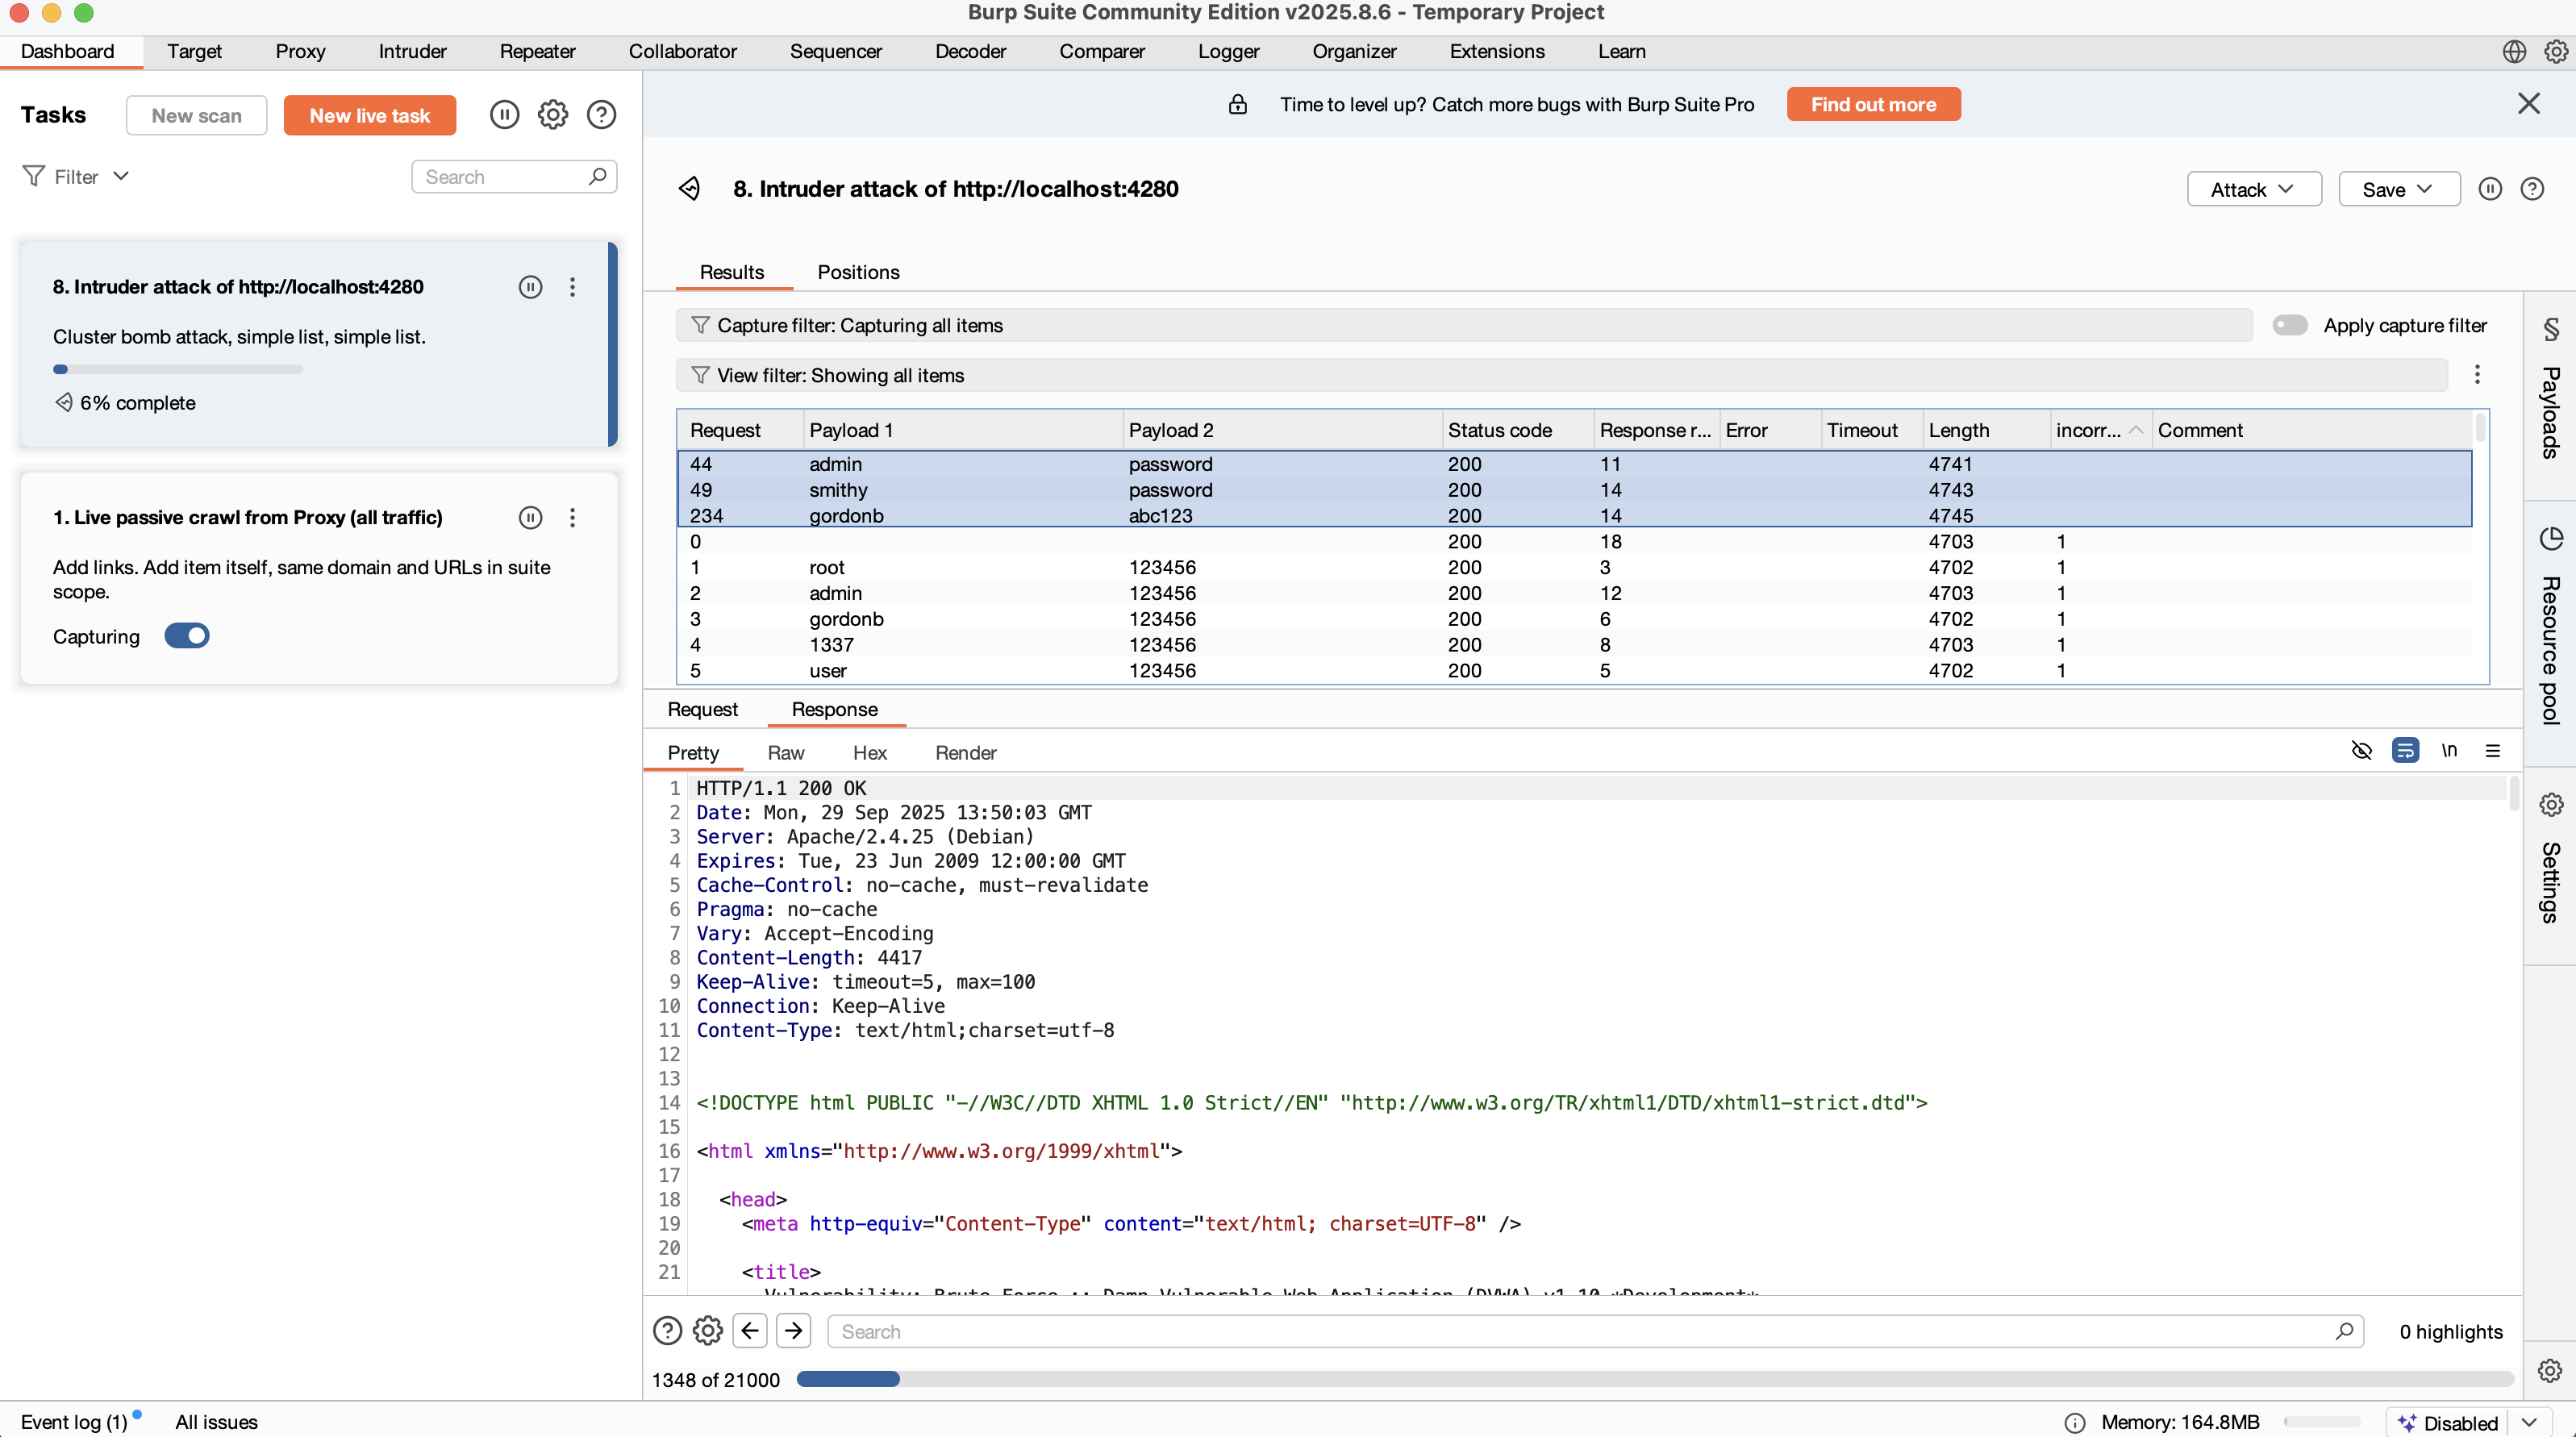
\includegraphics[width=1\linewidth]{Imagenes/brute_force_results.png}
    \caption{Resultados usernames y password}
    \label{fig:placeholder}
\end{figure}
\begin{itemize}
    \item \textbf{Username:} admin, \textbf{Password:} password
    \item \textbf{Username:} smithy, \textbf{Password:} password
    \item \textbf{Username:} gordonb, \textbf{Password:} abc123
\end{itemize}

\subsection{Obtención de código de inspect element (curl)}

A la hora de realizar una petición get, se envía un formulario con la información, para luego recibir la respuesta correspondiente, esto se puede capturar para replicar a través de la herramienta 'inspect' de nuestros navegadores.
Dentro de esta herramienta se abrirá la pestaña ´Network', en este apartado se capturan todas las comunicaciones efectuadas a través de los diferentes protocolos utilizados, en particular, si ahora enviamos una petición podremos ver como aparece en el apartado observado.
\begin{figure}[H]
    \centering
    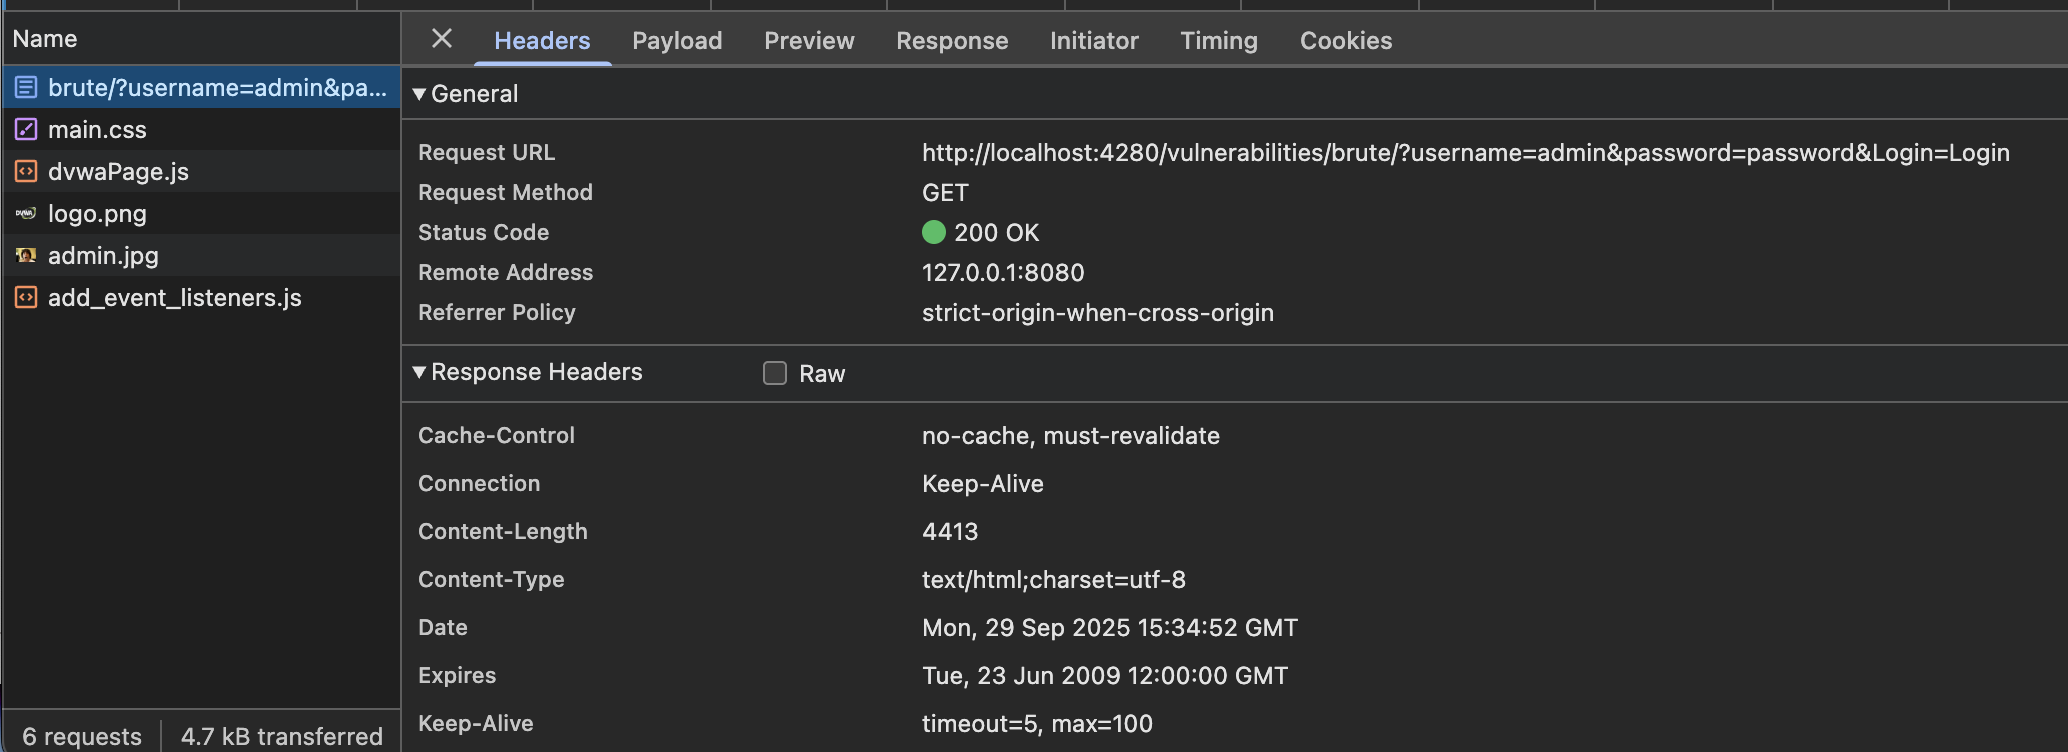
\includegraphics[width=1\linewidth]{Imagenes/cURL_how_to_obtain.png}
    \caption{Formulario obtenido}
    \label{fig:placeholder}
\end{figure}
En este caso se hizo una petición con el username 'admin' y la password 'password', se puede identificar cual es el formulario enviado ya que este contene los parámetros usados y un payload, de esta manera identificándolo, se puede pasar a obtener el cURL haciendo click derecho sobre esto y copiando cURL.
\begin{figure}[H]
    \centering
    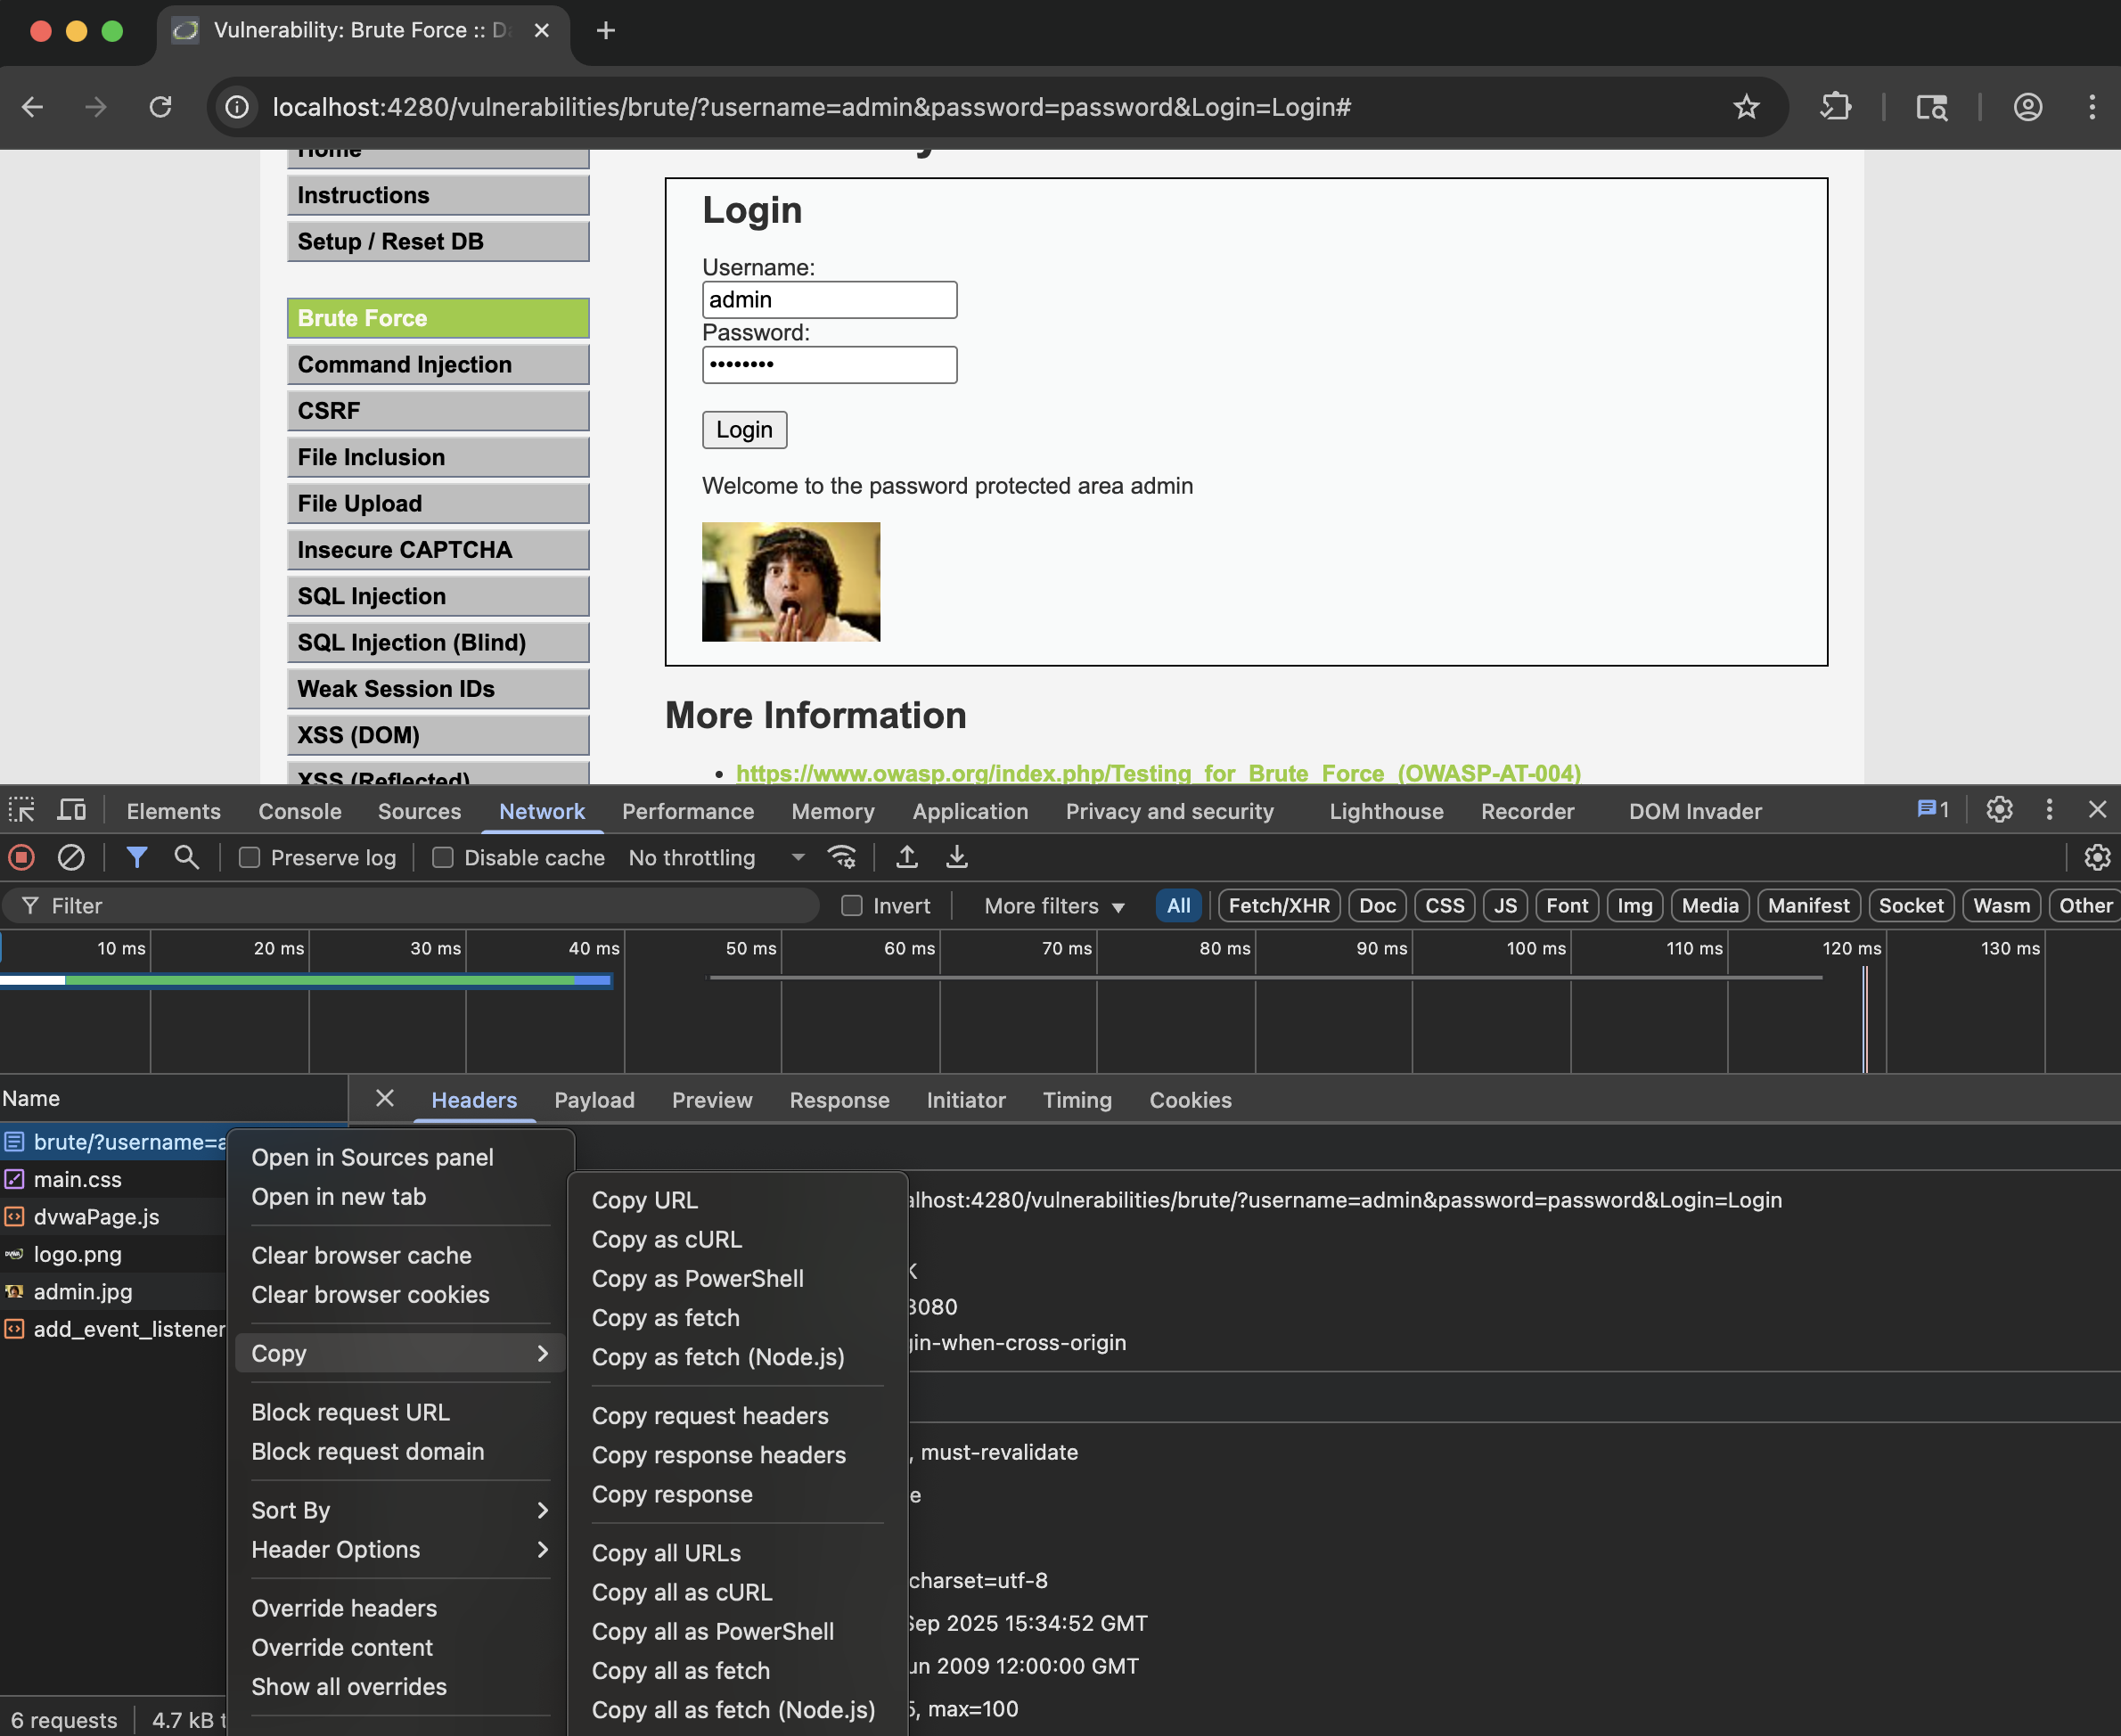
\includegraphics[width=0.65\linewidth]{Imagenes/cURL_obtain_valid.png}
    \caption{Obtención de cURL de una petición valida (username='admin', password='password')}
    \label{fig:placeholder}
\end{figure}
\begin{lstlisting}[language=bash, caption={cURL de petición válida}]
curl 'http://localhost:4280/vulnerabilities/brute/?username=admin&password=password&Login=Login' \
  -H 'Accept: text/html,application/xhtml+xml,application/xml;q=0.9,image/avif,image/webp,image/apng,*/*;q=0.8,application/signed-exchange;v=b3;q=0.7' \
  -H 'Accept-Language: en-US,en;q=0.9' \
  -b 'PHPSESSID=v7v1oj6anuh0mqbuacogscfp15; security=low' \
  -H 'Proxy-Connection: keep-alive' \
  -H 'Referer: http://localhost:4280/vulnerabilities/brute/?username=smithy&password=password&Login=Login' \
  -H 'Sec-Fetch-Dest: document' \
  -H 'Sec-Fetch-Mode: navigate' \
  -H 'Sec-Fetch-Site: same-origin' \
  -H 'Sec-Fetch-User: ?1' \
  -H 'Upgrade-Insecure-Requests: 1' \
  -H 'User-Agent: Mozilla/5.0 (Macintosh; Intel Mac OS X 10_15_7) AppleWebKit/537.36 (KHTML, like Gecko) Chrome/140.0.0.0 Safari/537.36' \
  -H 'sec-ch-ua: "Not=A?Brand";v="24", "Chromium";v="140"' \
  -H 'sec-ch-ua-mobile: ?0' \
  -H 'sec-ch-ua-platform: "macOS"'
\end{lstlisting}

\begin{figure}[H]
    \centering
    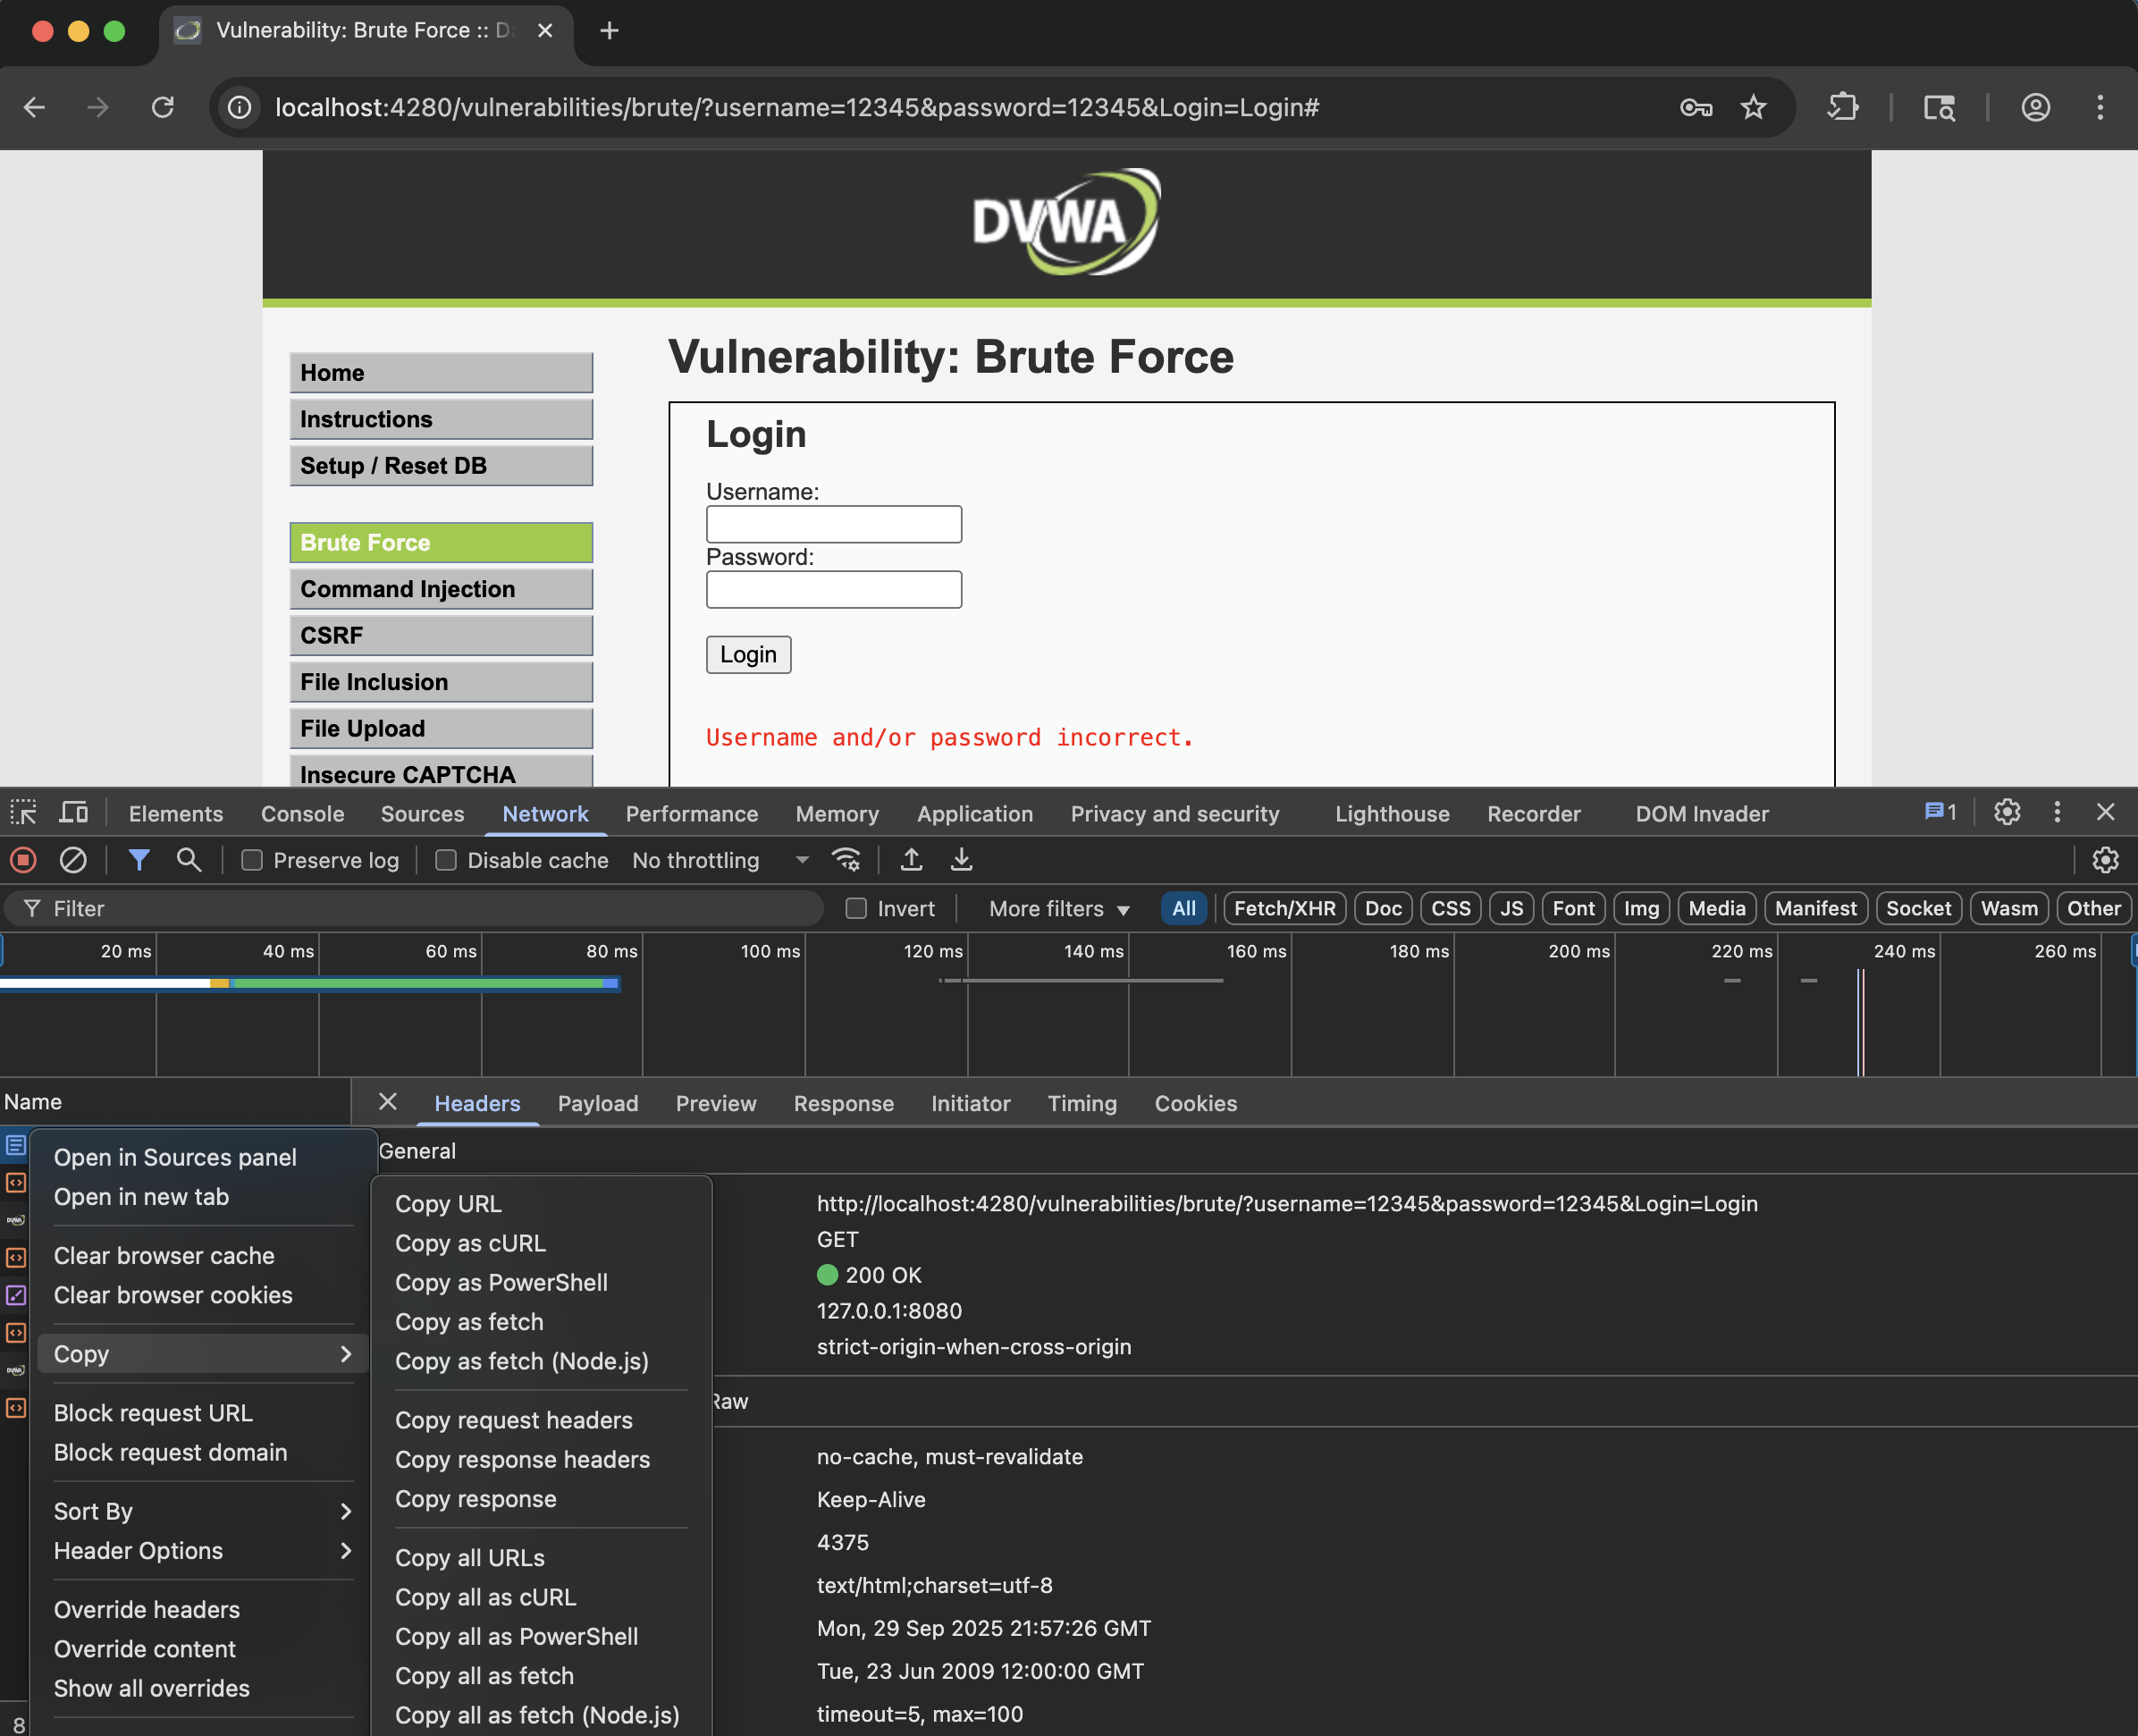
\includegraphics[width=0.65\linewidth]{Imagenes/cURL_obtain_invalid.png}
    \caption{Obtención de cURL de una petición inválida (username='12345', password='12345')}
    \label{fig:placeholder}
\end{figure}
\begin{lstlisting}[language=bash, caption={cURL de petición inválida}]
curl 'http://localhost:4280/vulnerabilities/brute/?username=12345&password=12345&Login=Login' \
  -H 'Accept: text/html,application/xhtml+xml,application/xml;q=0.9,image/avif,image/webp,image/apng,*/*;q=0.8,application/signed-exchange;v=b3;q=0.7' \
  -H 'Accept-Language: en-US,en;q=0.9' \
  -b 'PHPSESSID=v7v1oj6anuh0mqbuacogscfp15; security=low' \
  -H 'Proxy-Connection: keep-alive' \
  -H 'Referer: http://localhost:4280/vulnerabilities/brute/?username=admin&password=password&Login=Login' \
  -H 'Sec-Fetch-Dest: document' \
  -H 'Sec-Fetch-Mode: navigate' \
  -H 'Sec-Fetch-Site: same-origin' \
  -H 'Sec-Fetch-User: ?1' \
  -H 'Upgrade-Insecure-Requests: 1' \
  -H 'User-Agent: Mozilla/5.0 (Macintosh; Intel Mac OS X 10_15_7) AppleWebKit/537.36 (KHTML, like Gecko) Chrome/140.0.0.0 Safari/537.36' \
  -H 'sec-ch-ua: "Not=A?Brand";v="24", "Chromium";v="140"' \
  -H 'sec-ch-ua-mobile: ?0' \
  -H 'sec-ch-ua-platform: "macOS"'
\end{lstlisting}

\subsection{Utilización de curl por terminal (curl)}

Primero para utilizar cURL se verifica que esté instalado en el sistema, a través de:
\begin{lstlisting}[language=bash, caption={verión de cURL}]
curl --version
\end{lstlisting}
\begin{figure}[H]
    \centering
    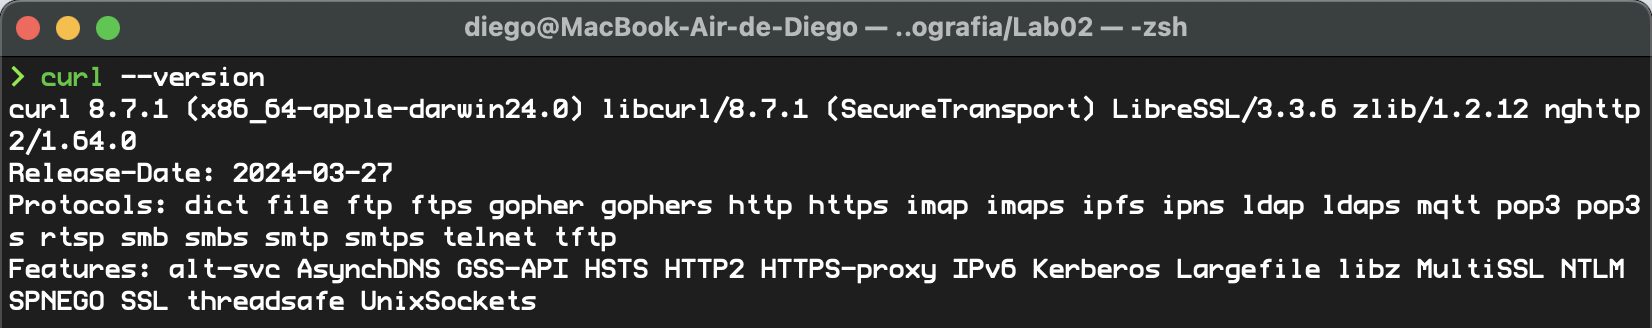
\includegraphics[width=1\linewidth]{Imagenes/cURL_version.png}
    \caption{versión de cURL}
    \label{fig:placeholder}
\end{figure}
Una vez tenemos esta verificación hecha, se pueden ejecutar los comandos cURL obtenidos en el paso anterior, obteniendo a través de la ejecución de este, el html respuesta de la petición hecha.
\begin{itemize}
    \item \textbf{Petición válida}
    \begin{figure}[H]
        \centering
        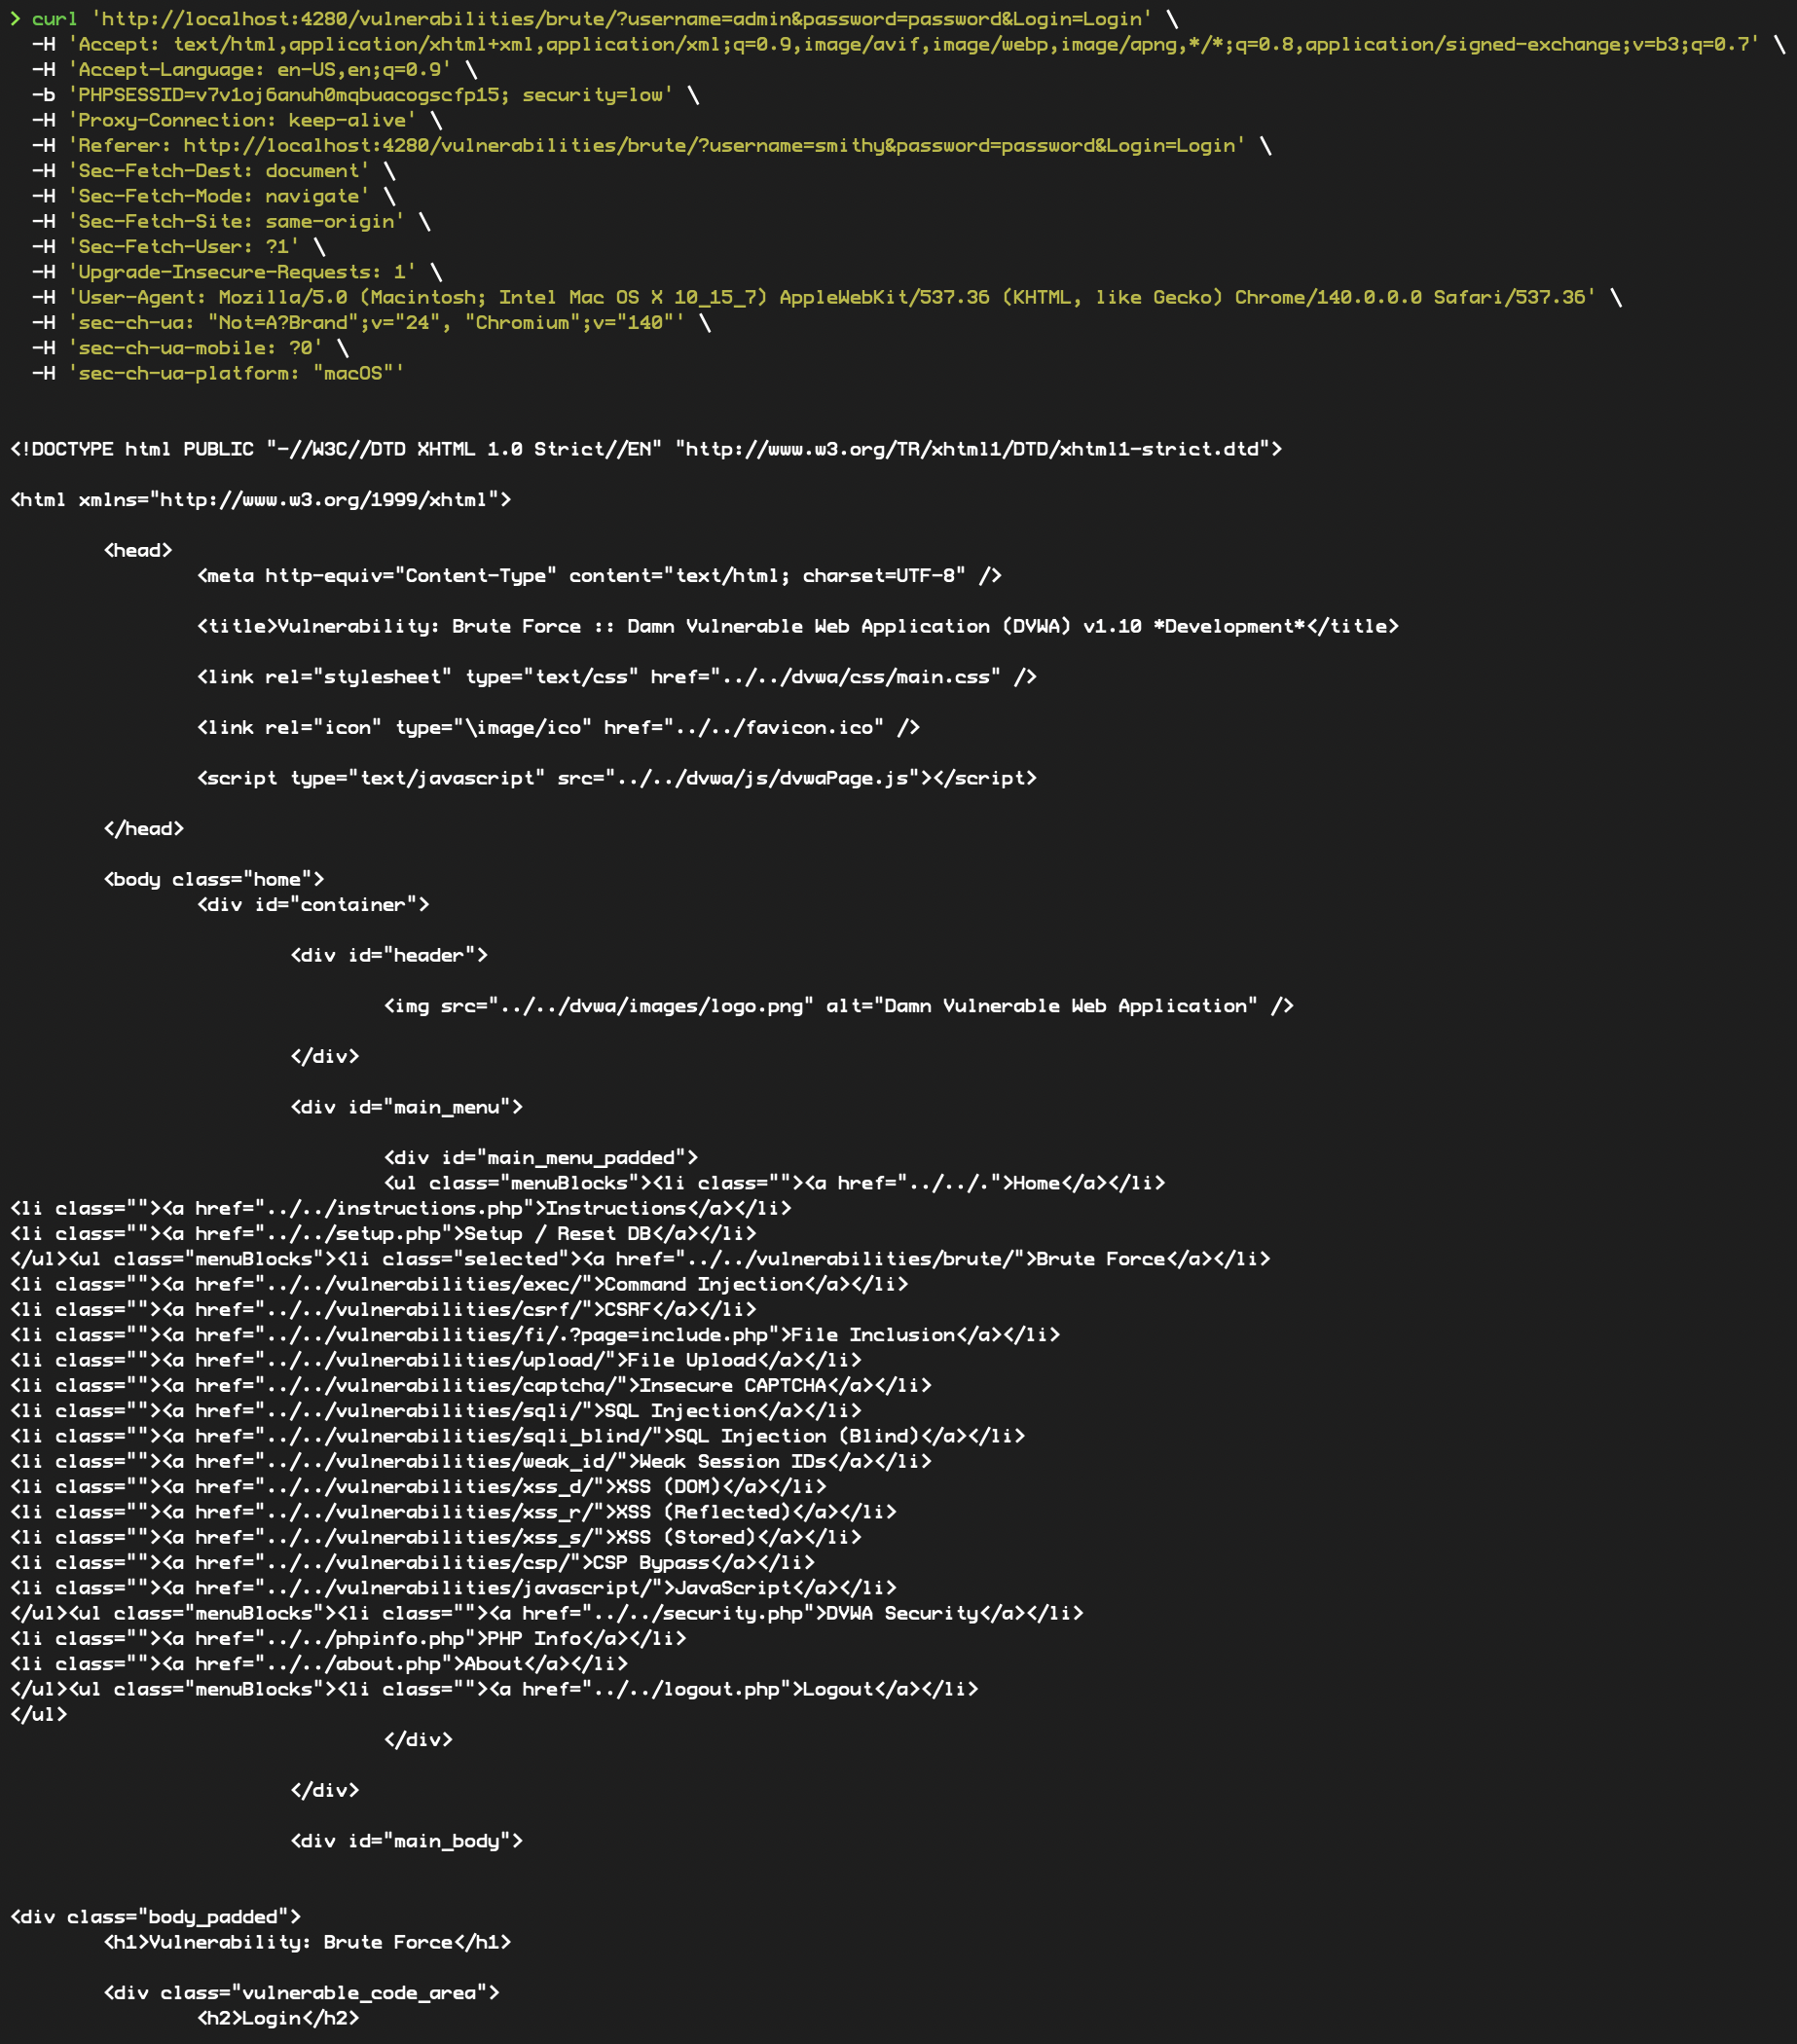
\includegraphics[width=1\linewidth]{Imagenes/cURL_valid_p1.png}
        \caption{Respuesta de petición válida parte 1}
        \label{fig:placeholder}
    \end{figure}
    \begin{figure}[H]
        \centering
        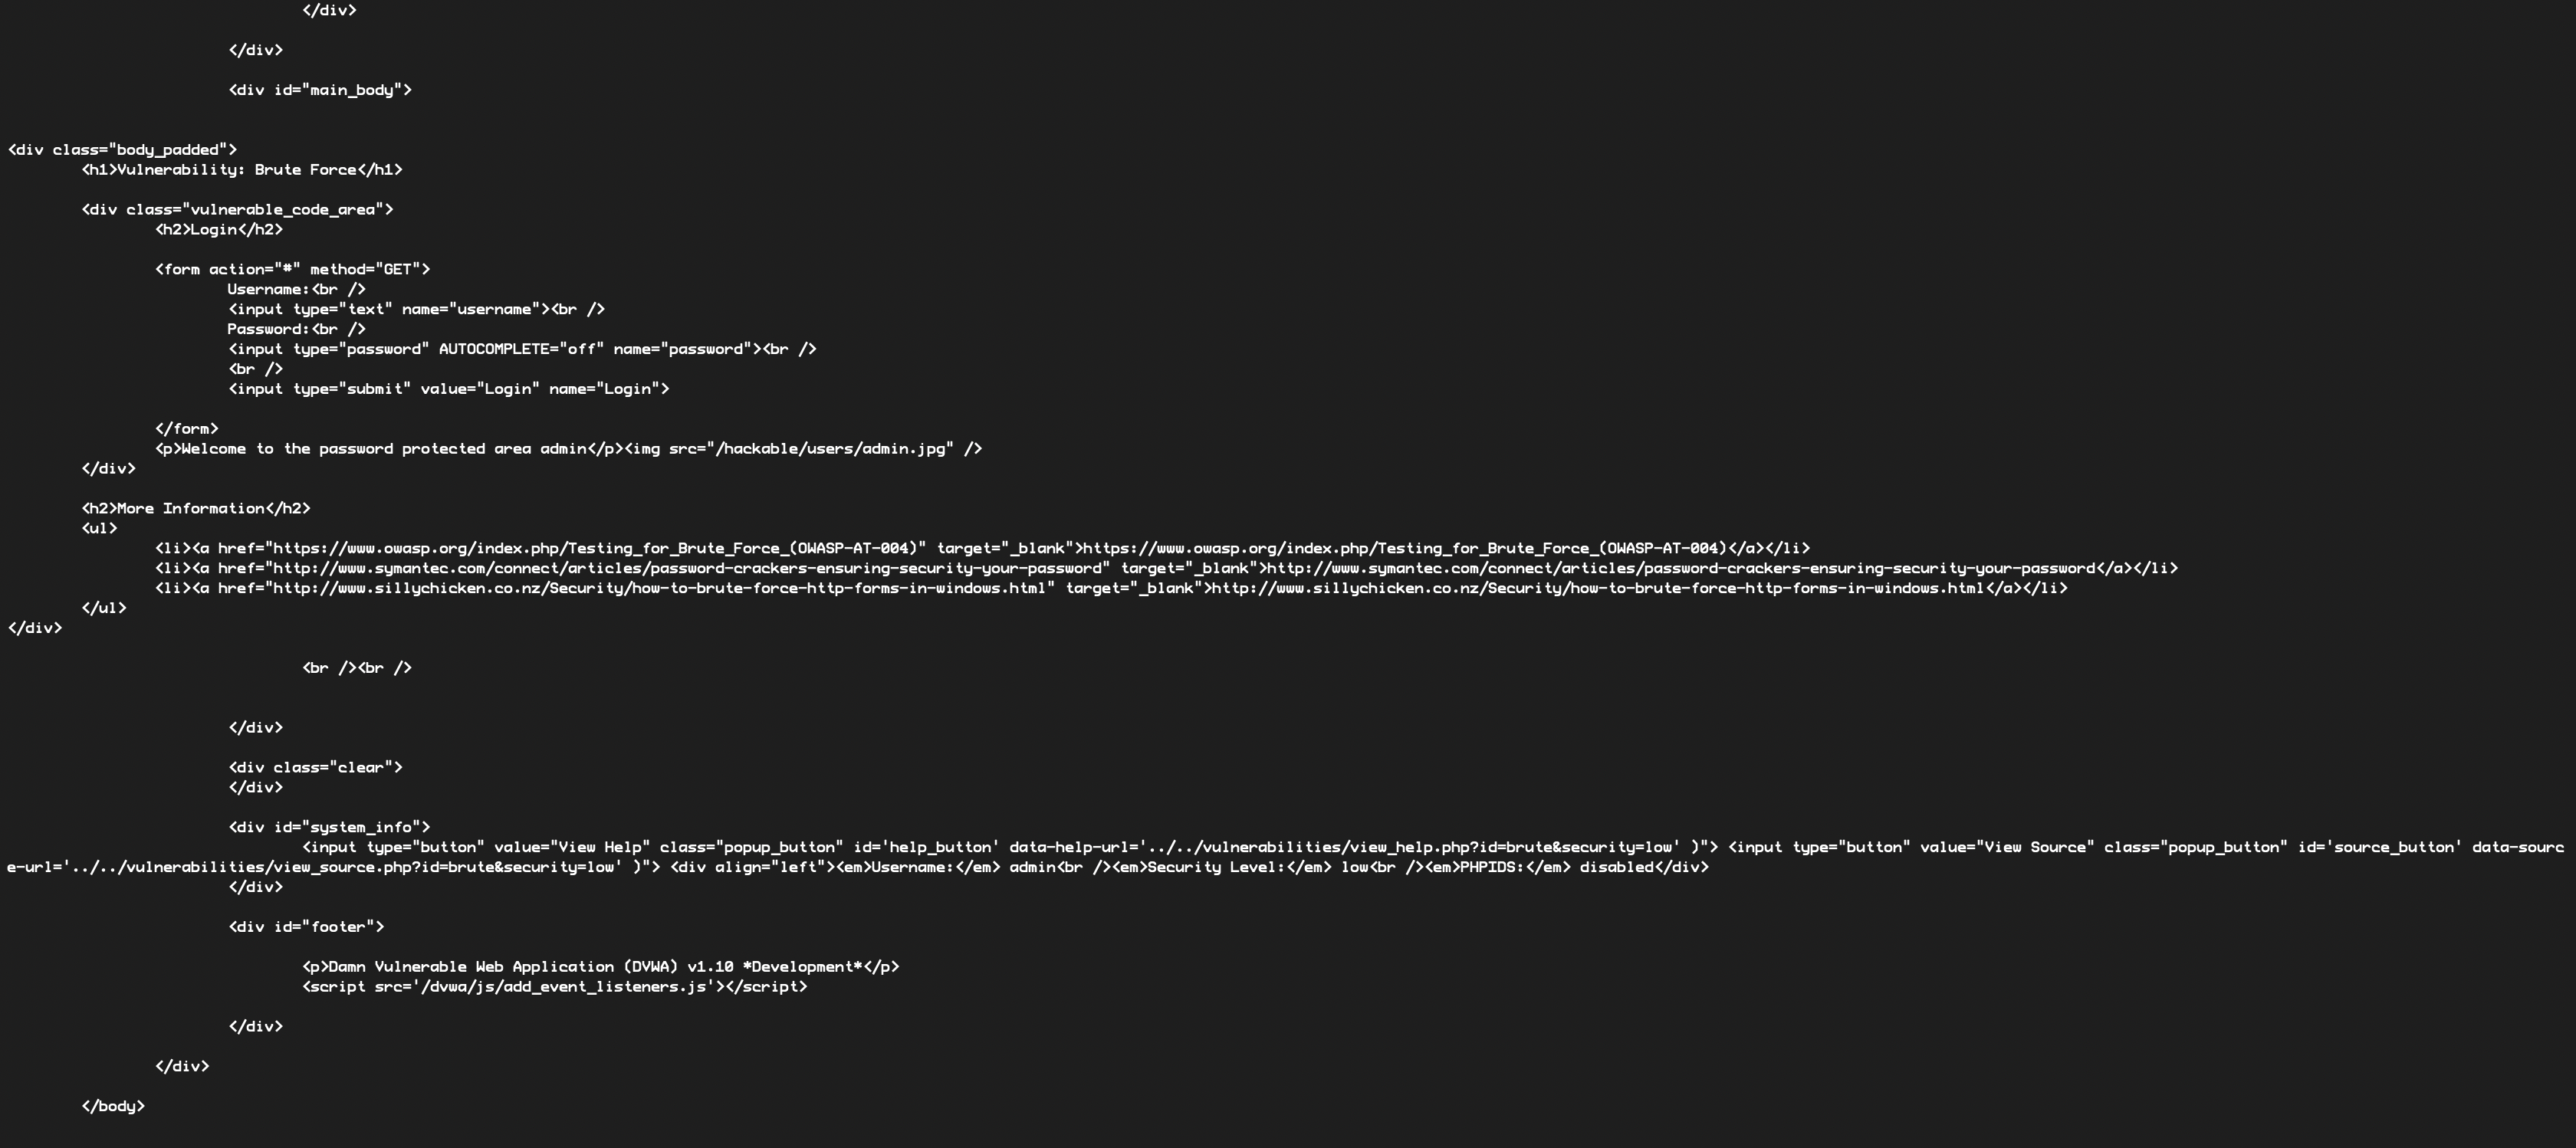
\includegraphics[width=1\linewidth]{Imagenes/cURL_valid_p2.png}
        \caption{Respuesta de petición válida parte 2}
        \label{fig:placeholder}
    \end{figure}
    \item \textbf{Petición inválida}
    \begin{figure}[H]
        \centering
        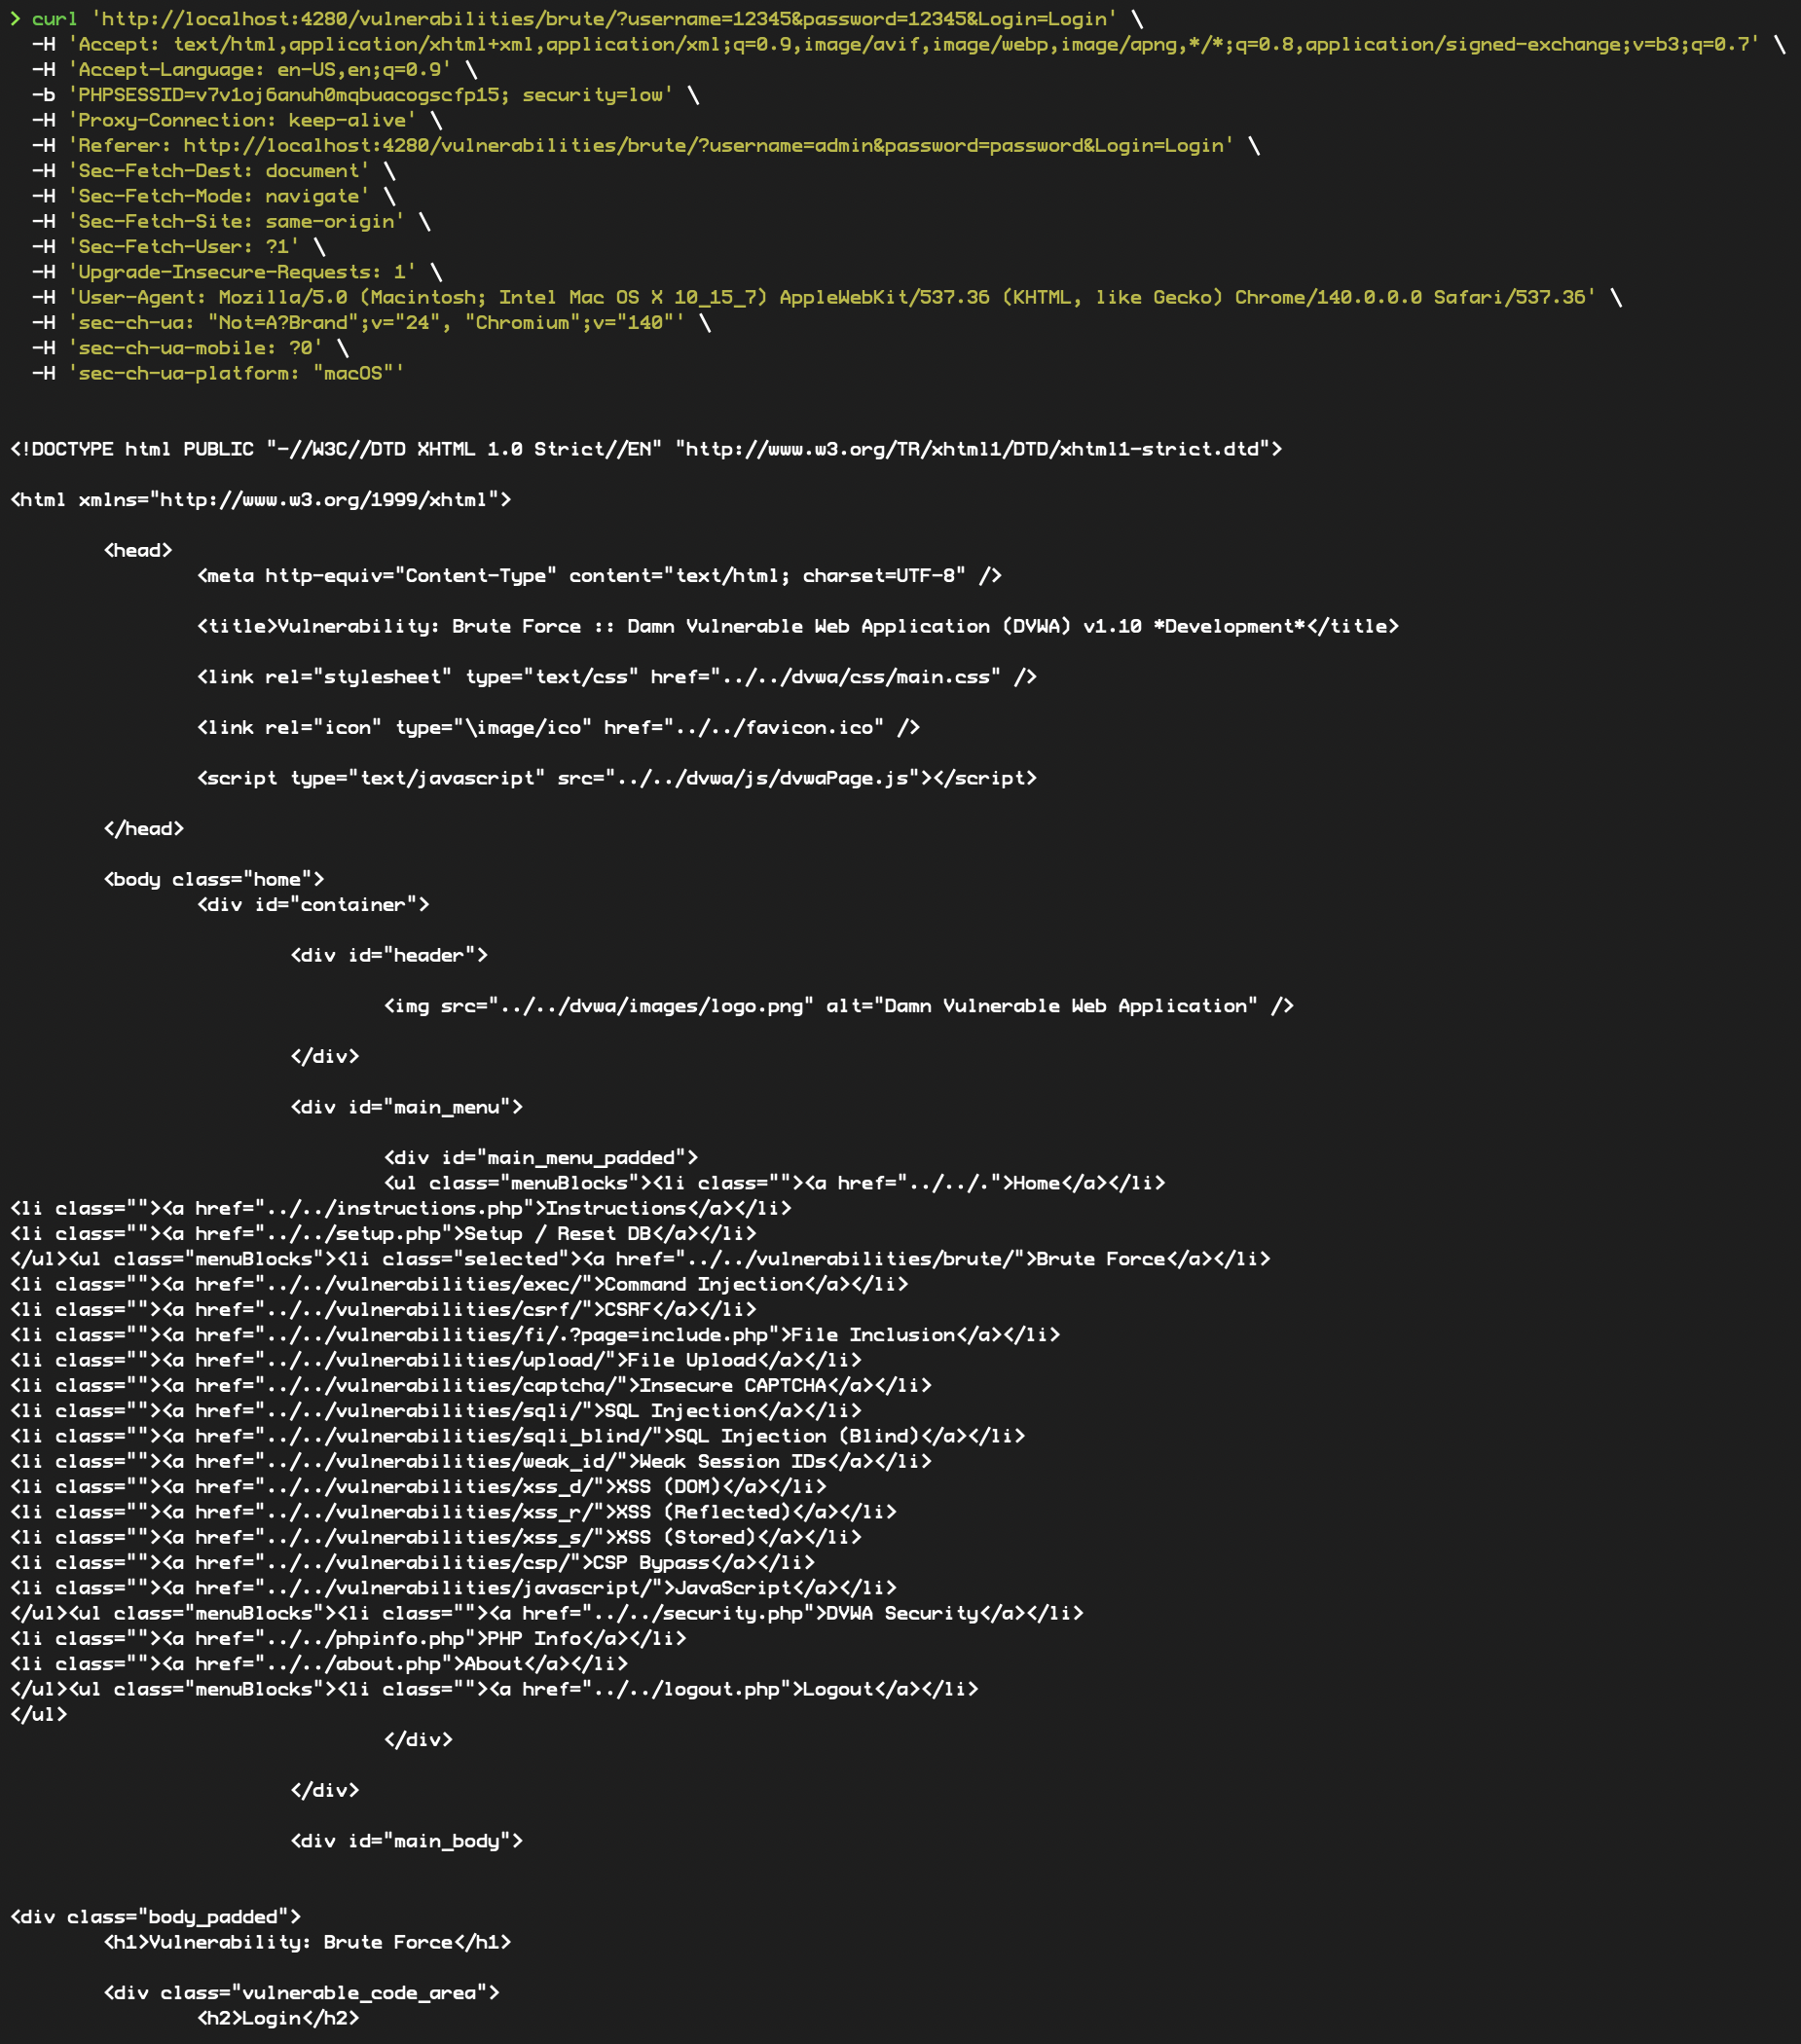
\includegraphics[width=1\linewidth]{Imagenes/cURL_invalid_p1.png}
        \caption{Respuesta de petición inválida parte 1}
        \label{fig:placeholder}
    \end{figure}
    \begin{figure}[H]
        \centering
        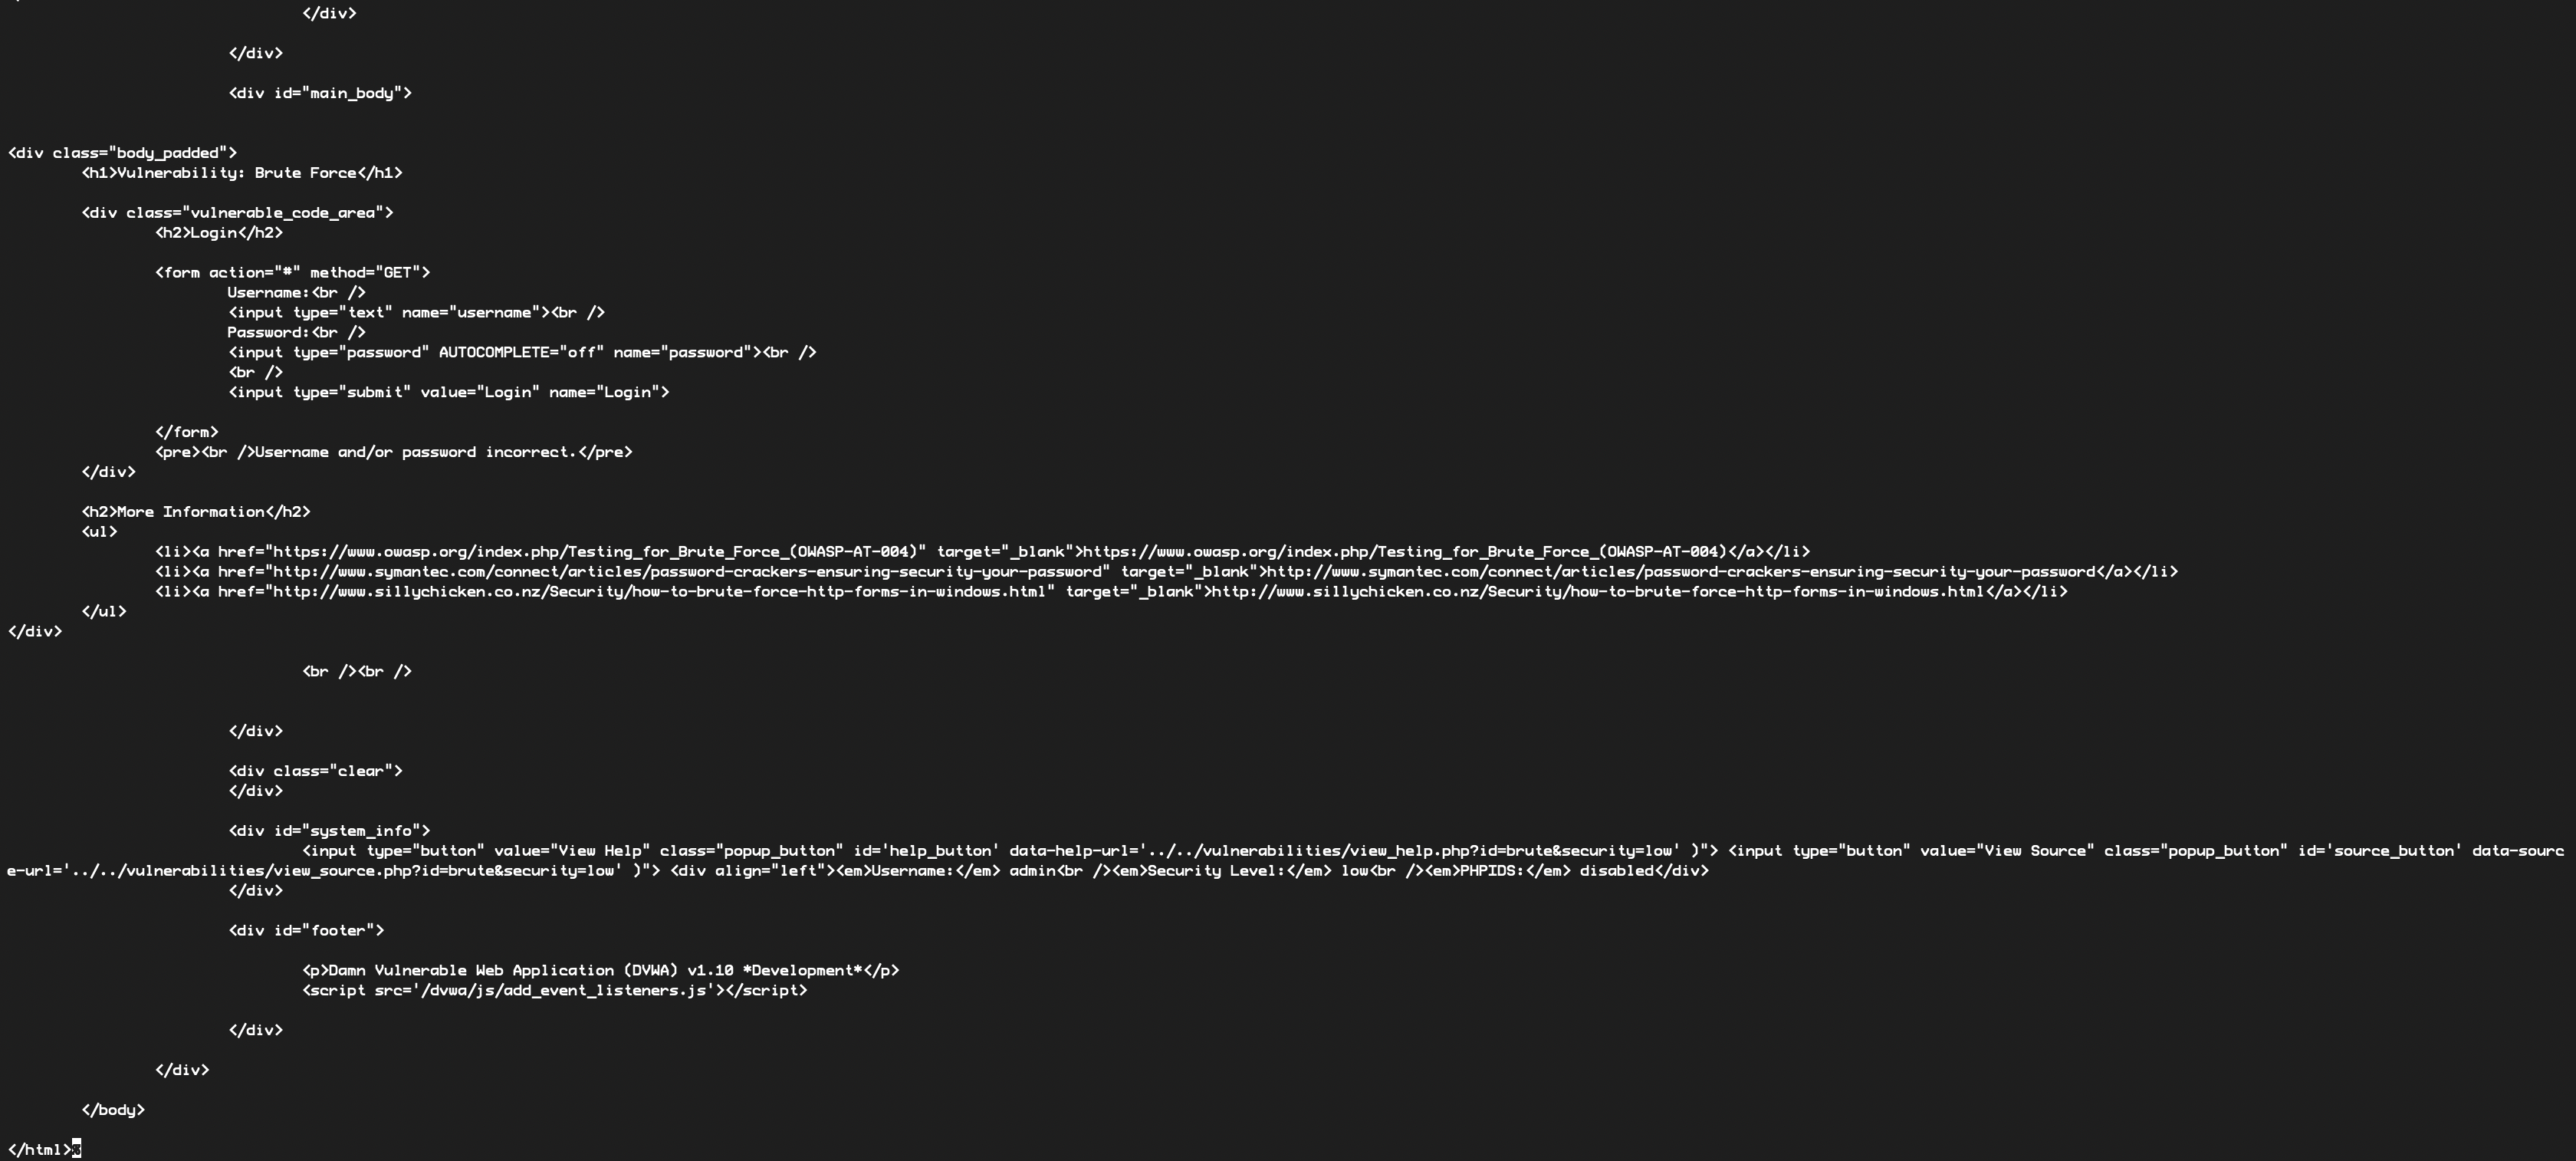
\includegraphics[width=1\linewidth]{Imagenes/cURL_invalid_p2.png}
        \caption{Respuesta de petición inválida parte 2}
        \label{fig:placeholder}
    \end{figure}
\end{itemize}

\subsection{Demuestra 4 diferencias (curl)}

Entre estas dos respuestas las principales diferencias encontradas fueron:
\begin{enumerate}
    \item \textbf{Mensaje de Respuesta:} Lo más notorio es el mensaje que cambia según si es un usuario válido y se pudo hacer el ingreso o si está erróneo, utilizando 'Username and/or password incorrect' si no se encontró un usuario, y usando 'Welcome...' y un mensaje personalizado para cada usuario si este existe.
    \item \textbf{Utilización de usuario en respuesta:} Cuando se hace un ingreso con las claves correctas, este entrega un mensaje en el cual se puede observar el usuario ingresado y varía según este, sin embargo cuando se ingresan valores incorrectos, responde con un mensaje predefinido, de esta manera no expone si existe o no tal usuario.
    \item \textbf{Largo del mensaje:} Punto directamente relacionado a la respuesta obtenida, ya que al utilizar distintos mensajes, se puede identificar a través de los carácteres si se cuenta con un resultado éxitoso o fallido.
    \item \textbf{Uso de imagen:} A la hora de hacer un loggeo exitoso, este aparece con una imagen relacionada al usuario, mientras que el intento erróneo no, esta información puede ser útil para entender lo que está pasando sin necesidad de mirar mensaje por mensaje o nisiquiera la captura.
\end{enumerate}

\subsection{Instalación y versión a utilizar (hydra)}

La instalación de hydra a través de consola para macbook es bastante sencillo, solo se requiere de tener instalado Homebrew, para luego ejecutar:
\begin{lstlisting}[language=bash, caption={Instalación de hydra}]
brew install hydra
\end{lstlisting}
Posterior a esto, se ejecuta el siguiente comando para obtener la versión instalada junto a otra información correspondiente a hydra.
\begin{lstlisting}[language=bash, caption={Versión de hydra}]
hydra -h
\end{lstlisting}
\begin{figure}[H]
    \centering
    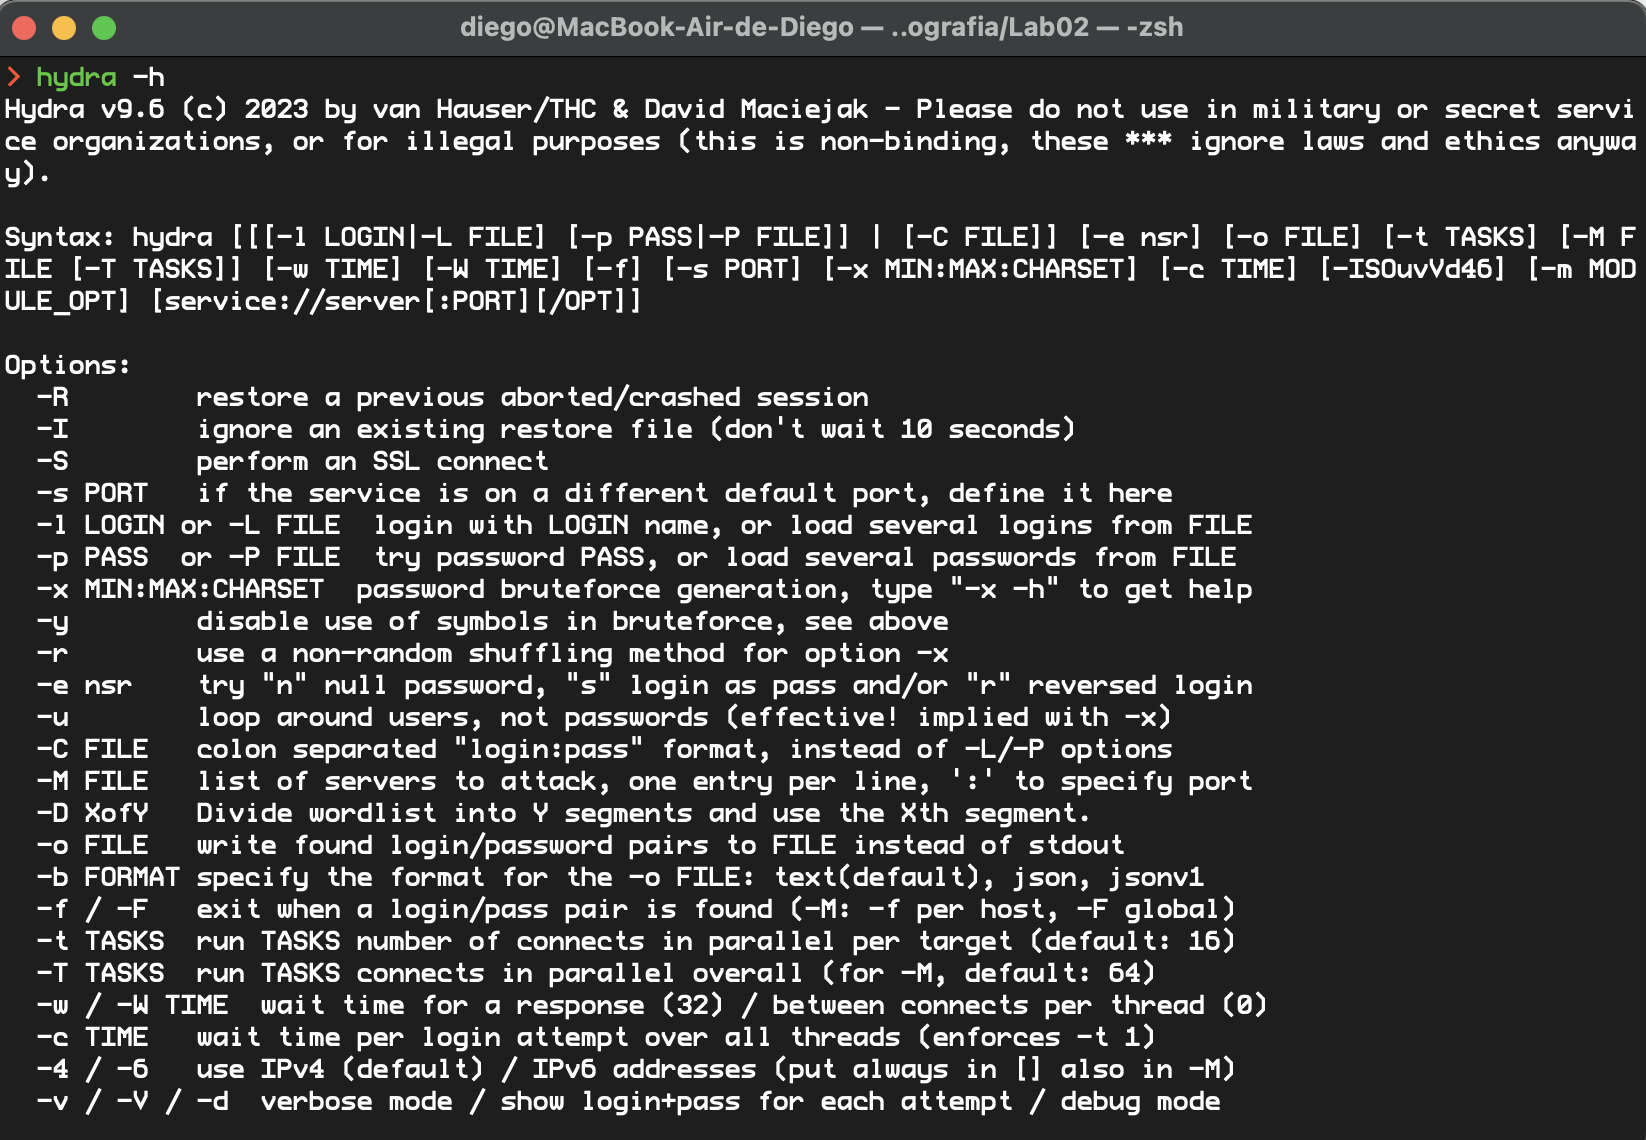
\includegraphics[width=0.5\linewidth]{Imagenes/hydra_version.png}
    \caption{Versión e información adicional de hydra}
    \label{fig:placeholder}
\end{figure}

\subsection{Explicación de comando a utilizar (hydra)}

\subsection{Obtención de al menos 2 pares (hydra)}

\subsection{Explicación paquete curl (tráfico)}

\subsection{Explicación paquete burp (tráfico)}

\subsection{Explicación paquete hydra (tráfico)}

\subsection{Mención de las diferencias (tráfico)}

\subsection{Detección de SW (tráfico)}

\subsection{Interacción con el formulario (python)}

\subsection{Cabeceras HTTP (python)}

\subsection{Obtención de al menos 2 pares (python)}

\subsection{Comparación de rendimiento con Hydra, Burpsuite, y cURL (python)}

\newpage
\subsection{Demuestra 4 métodos de mitigación (investigación)}

% Please add the following required packages to your document preamble:
%\begin{table}[htbp]

\section*{Conclusiones y comentarios}

\end{document}
